% 									CPE - Vorlage für Elektrotechnik
%                   					      2023 HTL Weiz
%----------------------------------------------------------------------------------------------------
% Dieses \LaTeX Template kann als Grundlage für die Erstellung von Dokumentationen verwendet werden.
% In diesem File werden sämtliche Einstellungen, sowie die einzelnen Inhalte miteinander verknüpft.
%----------------------------------------------------------------------------------------------------

%****************************************************************************************************
%=========================== D O K U M E N T  I N F O R M A T I O N E N =============================
%****************************************************************************************************
% Hier werden einheitliche Infromationen für das Dokument festgelegt. (selbst ausfüllen)

\newcommand{\iYear}{2023/24}																			% Jahrgang
\newcommand{\iDate}{10.04.2024}																			% Datum
\newcommand{\iLUName}{Zeitnehmung}																		% Übungsname
\newcommand{\iClass}{5AHET}																				% Klasse
\newcommand{\iNameOne}{Jonas Bichler}																	% Schüler
\newcommand{\iNumber}{1}																				% Klassenbuchnummer
\newcommand{\iCoachOne}{Prof. DI. Bergler Ewald}														% Lehrperson 1
\newcommand{\iCoachTwo}{}																				% Lehrperson 2

%****************************************************************************************************
%=========================== D O K U M E N T  E I N S T E L L U N G E N =============================
%****************************************************************************************************
% Hier werden die Textart, das Papier, die Schriftgröße und alle Pakete definiert.

\documentclass[12pt, a4paper, ngerman] {scrartcl}														% Papierformat
% 							Package-File - Vorlage für Elektrotechnik
%                    					    2023 HTL Weiz
%----------------------------------------------------------------------------------------------------
% Dieses \LaTeX Template kann als Grundlage für die Erstellung von Diplomarbeitsdokumentationen
% verwendet werden. In diesem File werden sämtliche Pakete eingebunden. 
%----------------------------------------------------------------------------------------------------

%=========================================== P A K E T E ============================================

\usepackage[onehalfspacing]{setspace}																	% Formatierung
\usepackage[usenames, dvipsnames,svgnames,table]{xcolor}												% Tabellen + Farbe
\usepackage[utf8x]{inputenc}																			% Codierung (ASCII, ISO)
\usepackage[ngerman]{babel}																				% Sprache
\usepackage{fancyhdr}																					% Aussehen
\usepackage[T1]{fontenc}																				% Aussehen
\usepackage[scaled]{uarial}																				% Schriftart: Arial (skaliert)
\renewcommand*\familydefault{\sfdefault}																% Standardschriftart
\usepackage[backend=biber, citestyle=numeric, bibstyle=numeric]{biblatex}								% Zitierungen und Literatur
\addbibresource{bibliography.bib}																		% Bib-Datei
\usepackage{hyperref}																					% Quicklink Referenz fuer Literatur
\usepackage{float}																						% Grafiken strukturieren
\usepackage{amsmath}																					% Mathematik
\usepackage{amsfonts}																					% Mathematik
\usepackage{amsthm}																						% Mathematik
\usepackage{amssymb}                    																% Mathematik-Symbole
\usepackage{amsbsy}																						% Mathematik-Symbole
\usepackage{mathrsfs}                   																% Symbole fuer Fourier und Laplace Transformation
\usepackage{calc}																						% Arithmetische Rechenoperationen
\usepackage{eufrak}                     																% Fraktur Symbole
\usepackage{array,longtable,calc,amsmath}																% Tabellen und Mathematik
\usepackage{multirow}																					% Tabellen
\usepackage{longtable}																					% Tabellen
\usepackage{array}																						% Tabellen
\usepackage{tabulary}																					% Tabellen
\usepackage{tabularx}																					% Tabellen
\usepackage{caption}																					% Textformatierung
\usepackage{ifthen}																						% Textformatierung
\usepackage{sidecap}																					% Textformatierung
\usepackage{subcaption}																					% Textformatierung
\usepackage{tikz}																						% Textformatierung
\usepackage{wrapfig}   																					% Textformatierung
\usepackage{titling}																					% Textformatierung
\usepackage{textfit}																					% Textformatierung
\usepackage{chngpage}																					% Textformatierung
\usepackage{lastpage}																					% Textformatierung
\usepackage{setspace}																					% Formatierung
\usepackage{xspace}																						% Formatierung
\usepackage{listings}																					% Codedarstellung
\usepackage{docmute}																					% Datei-Strukturierung
\usepackage{pdfpages}																					% PDF in Latexdokument einfuegen
\usepackage{graphicx}																					% Grafiken
\graphicspath{{./../03_Graphics/}}																		% Grafikenpfad
\usepackage{color}																						% Farben
\usepackage{tcolorbox}																					% Textfelder
\usepackage{scrkbase}																					% Artikelformat
\usepackage{upgreek}																					% Griechische Buchstaben
\usepackage{textgreek}																					% Griechische Buchstaben
\usepackage[printonlyused, withpage]{acronym}															% Akronyme (Abkuerzungen)
\usepackage[acronym,toc]{glossaries}																	% Sprachuebersetzung
\usepackage{enumitem}
\usepackage{adjustbox}
\usepackage{comment}

%============================== M A T H E M A T I K  S Y M B O L E ====================================

\renewcommand{\j}{\ensuremath{\mathrm{j}}} 																% Imaginäere Einheit
\newcommand{\conj}[1]{\ensuremath{{#1}^\ast}} 															% Komplex Konjugiert
\renewcommand{\c}[1]{\ensuremath{\boldsymbol{#1}}} 														% Komplex Fettdruck
%
\newcommand{\E}[1]{\ensuremath{\mathrm{E}\{ {#1} \}}} 													% Expectation E{*}
%
\newcommand{\F}[1]{\ensuremath{\mathcal{F}\{ {#1} \}}} 													% Fourier F{*}
\newcommand{\Fi}[1]{\ensuremath{\mathcal{F}^{-1}\{ {#1} \}}}										 	% Fourier F{*}
%
\renewcommand{\L}[1]{\ensuremath{\mathcal{L}\{ {#1} \}}} 												% Laplace F{*}
\newcommand{\Li}[1]{\ensuremath{\mathcal{L}^{-1}\{ {#1} \}}} 											% Laplace F{*}
%
\newcommand{\e}[1]{\ensuremath{\mathrm{e}^{#1}}} 														% Exponential e^*
%
\renewcommand{\o}[1]{\ensuremath{\overline{#1}}} 														% Overline
%
\newcommand{\abs}[1]{\ensuremath{ | {#1} | }} 															% Absolut |a|
\newcommand{\norm}[1]{\ensuremath{ \| {#1} \| }} 														% Norm ||a||
\newcommand{\avg}[1]{\ensuremath{ < {#1} > }} 															% Zeitintervall <a>
\newcommand{\sign}{\ensuremath{\mathrm{sign}\,}} 														% Signum Funktion
%
\newcommand{\N}[1]{\ensuremath{\mathbb{N}}} 															% Natuerliche Zahlen
\newcommand{\R}[1]{\ensuremath{\mathbb{R}}} 															% Rationale Zahlen
\newcommand{\C}[1]{\ensuremath{\mathbb{C}}} 															% Komplexe Zahlen
\newcommand{\Z}[1]{\ensuremath{\mathbb{Z}}} 															% Ganze Zahlen
\newcommand{\Q}[1]{\ensuremath{\mathbb{Q}}} 															% Irrationale Zahlen
%
\newcommand{\inti}{\ensuremath{\int_{0}^{\,\infty}}} 													% int 0 to infty
\newcommand{\intii}{\ensuremath{\int_{-\infty}^{\,\infty}}} 											% int -infty to infty
\newcommand{\iintii}{\ensuremath{\iint_{-\infty}^{\quad\infty}}} 										% int -infty to infty

																% Packete

%****************************************************************************************************
%==================================== D E S I G N K O N Z E P T =====================================
%****************************************************************************************************
% Hier wird das grundsätzliche Aussehen des Dokuments festgelegt.

% 							Style-File - Vorlage für Elektrotechnik
%                         				2023 HTL Weiz
%----------------------------------------------------------------------------------------------------
% Dieses \LaTeX Template kann als Grundlage für die Erstellung von Diplomarbeitsdokumentationen
% verwendet werden. In diesem File wird das Aussehen, sowie Designeinstellungen implementiert.
%----------------------------------------------------------------------------------------------------

%****************************************************************************************************
%==================================== S E I T E N F O R M A T =======================================
%****************************************************************************************************

\usepackage[a4paper, left=2.5cm, right=2.5cm, top=2.5cm, bottom=2.5cm]{geometry}						% A4 und Seitenränder
\setlength{\textwidth}{16.0cm}																			% Textbreite
\setlength{\parindent}{0pt}																				% Einzug ausschalten
\setstretch{1.3}																						% Zeilenabstand
\pagestyle{fancy}																						% Seitenformatierung
\setlist[itemize,enumerate]{itemsep=0pt}
\setlength{\parindent}{0pt}
%****************************************************************************************************
%=============================== K O P F-  U N D  F U ß Z E I L E ===================================
%****************************************************************************************************

%======================================== S T A N D A R D ===========================================

% Kopfzeile
\lhead{\LARGE Zero Emission Challenge}						% Baselineskip entfernen falls der Übungsname in eine Zeile passt und das Logo kleiner machen
\rhead{\vspace{-8pt}
\includegraphics[scale=0.3]{./00_Introduction/ZeroEmission-Logo.jpg}}
\renewcommand{\headrulewidth}{0.4pt}

% Fußzeile
\lfoot{\iNameOne}
\cfoot{\iYear}
\rfoot{Seite \thepage\ von \pageref{LastPage}}
\renewcommand{\footrulewidth}{0.4pt}

%****************************************************************************************************
%==================================== F A R B E N F O R M A T =======================================
%****************************************************************************************************

\definecolor{kaki}{rgb}{0.74,0.74,0.088}
\definecolor{dred}{rgb}{0.722,0.18,0.18}
\definecolor{darkgrey}{rgb}{0.364,0.411,0.439}
\definecolor{lightgrey}{rgb}{0.776,0.792,0.803}
\definecolor{pythonkeyword}{HTML}{0066CC}
\definecolor{stringstyle}{HTML}{FF5E05}
\definecolor{cppvariable}{HTML}{9CDCFE}
\definecolor{cppkeyword}{HTML}{0066CC}

%****************************************************************************************************
%=============================== G L I E D E R U N G S E B E N E N ==================================
%****************************************************************************************************

% \setcounter{secnumdepth}{5}																			% Gliederungstiefe (hier: 5. Unterüberschrift [1.1.1.1.1]) jedoch eher für "BOOK" geeignet
\setcounter{tocdepth}{2}																				% Inhaltsverzeichnistiefe (hier 2. Unterüberschrift [1.1])

%****************************************************************************************************
%============================== B I L D U N T E R S C H R I F T E N =================================
%****************************************************************************************************

\captionsetup{margin=10pt,font=small, labelfont={color=black!80, bf}, textfont={color=black!60}, format=hang, indention=-1cm}
\captionsetup[wrapfigure]{name=Abbildung}
\captionsetup[figure]{name=Abbildung}

%****************************************************************************************************
%================================= T E X T F E L D V O R L A G E ====================================
%****************************************************************************************************

\newenvironment{Textfeld1}{\begin{tcolorbox}[colback=lightgrey!5,colframe=darkgrey]\small}{\end{tcolorbox}}
\newenvironment{Textfeld2}{\begin{tcolorbox}[colback=lightgrey!5,colframe=blue]\small}{\end{tcolorbox}}

%****************************************************************************************************
%================================== C O D E D A R S T E L U N G =====================================
%****************************************************************************************************

%============================== S T R U K T U R I E R T E R  T E X T ================================

\lstdefinelanguage{Python}{
	keywords={and, as, assert, break, class, continue, def, del, elif, else, except, False, finally, for, from, global, if, import, in, is, lambda, None, nonlocal, not, or, pass, raise, return, True, try, while, with, yield},
	keywordstyle=\color{pythonkeyword},
	commentstyle=\color{green},
	stringstyle=\color{stringstyle},
	sensitive=true,
	comment=[l]{\#},
	morestring=[b]',
	morestring=[b]",
	keywords=[2]{SERVER\_IP, MQTT\_USER, MQTT\_PASSWORD, DB\_USER, DB\_PASSWORD},
	keywordstyle=[2]{\color{pythonkeyword}},
}

\lstdefinelanguage{myCpp}{
	language=C++,
	morekeywords={},
	keywordstyle=\color{cppkeyword},
	commentstyle=\color{green},
	stringstyle=\color{stringstyle},
	sensitive=true,
	comment=[l]{//},
	morecomment=[s]{/*}{*/},
	morestring=[b]",
	morekeywords=[2]{wifi\_ssid, wifi\_password, mqtt\_server, mqtt\_user, mqtt\_password},
	keywordstyle=[2]{\color{cppvariable}}
}

\lstset{
	basicstyle=\small\ttfamily,
	numbers=none,
	rulecolor=\color{black}, 
	numbersep=5pt,
	breaklines=true,
	breakatwhitespace=true,
	tabsize=4,
	columns=flexible,
	frame=none, 
	backgroundcolor=\color{darkgrey!10}
}




%****************************************************************************************************
%==================================== D O K U M E N T A T I O N =====================================
%****************************************************************************************************
% Hier beginnt die eigentliche Dokumentation der Laborübung.

\begin{document}
%===================================== I N T R O D U C T I O N ======================================
% Hier wird die Einleitung des Dokuments abgehandelt und strukturiert. (selbst ausfüllen)

% 								Einleitung - Vorlage für Elektrotechnik
%                         					2023 HTL Weiz
%----------------------------------------------------------------------------------------------------
% Dieses \LaTeX Template kann als Grundlage für die Erstellung von Diplomarbeitsdokumentationen
% verwendet werden. In diesem File wird eine einheitliche Einleitung abgehandelt.
%----------------------------------------------------------------------------------------------------

%****************************************************************************************************
%====================================== T I T E L S E I T E =========================================
%****************************************************************************************************

%=========================== K O P F Z E I L E - T I T E L S E I T E ================================

\begin{titlingpage}
	%Kopfzeile
	\begin{figure}[h]
		\begin{minipage}{0.2\textwidth}
			\raggedright
			
\includegraphics[width=\linewidth]{./00_Introduction/HTL-Weiz-Logo.pdf}						% HTL-Weiz-Logo
		\end{minipage}
		\hfill
		\begin{minipage}{0.1\textwidth}
			\raggedleft
			
\includegraphics[width=\linewidth]{./00_Introduction/ZeroEmission-Logo.jpg}					% Zero-Emission-Logo
		\end{minipage}
		\hfill
		\begin{center}
			\vspace{-1.5cm}
			\centering
			\large \textbf{Höhere Technische\\ Bundeslehranstalt Weiz}									% HTBLA Weiz
		\end{center}
	\end{figure}
	
	\vspace{1cm}
	
	%========================== D O K U M E N T I N F O R M A T I O N E N ==============================
	
	\begin{center} {\resizebox{15.5cm}{1cm}{\textbf{Zero Emission Challenge}}}\\ \vspace{0.25cm} {\large Höhere Abteilung für Elektrotechnik}\\ \end{center}	% Diplomarbeit
	\noindent\rule{\textwidth}{0.4pt}
	\vspace{0.3cm}
	\begin{center} {\LARGE\textbf{\iLUName}}\\ \end{center}																							% Diplomarbeitsname
	\vspace{0.3cm}
	\noindent\rule{\textwidth}{0.4pt}
	
	\renewcommand{\arraystretch}{1.5}
	\begin{table}[H]
		\begin{tabular}{p{6cm} p{5cm} p{3.75cm}}
			\textbf{Abteilung}     & \textbf{Jahrgang} & \hspace{1cm} \textbf{Datum}  \\
			Elektrotechnik         & \iYear            & \hspace{1cm} \iDate          \\
			                       &                   &                              \\
			\textbf{Themenbereich} & \textbf{Schüler}  & \hspace{1cm} \textbf{Klasse} \\
			Hauptverantwortlicher  & Jonas Bichler     & \hspace{1cm} 5AHET           \\
			Webserver-Design       & Florian Puchegger & \hspace{1cm} 5AHET           \\
			Gehäuse-Konstruktion   & Rene Winter       & \hspace{1cm} 5AHET           \\
			Gehäuse-Konstruktion   & Thomas Pieber     & \hspace{1cm} 5AHET           \\
			Pegelwandler           & Fritz Stefan      & \hspace{1cm} 5AHET           \\
			ESP32-S2 \& GPS-Modul  & Ricardo Wolf      & \hspace{1cm} 5BHET           \\
			                       &                   &                              \\
			\textbf{Lehrpersonen}  &                   &                              \\
			\multicolumn{3}{l}{\iCoachOne}                                            \\
			\multicolumn{3}{l}{\iCoachTwo}
		\end{tabular}
	\renewcommand{\arraystretch}{1}
	\end{table}
\end{titlingpage}

\newpage
\tableofcontents
\newpage




%========================================== I N H A L T E ===========================================
% Hier wird die Aufgabenstellung implementiert. (selbst ausfüllen)

% 									Inhalte - Vorlage für Elektrotechnik
%                        					 2023 HTL Weiz
%----------------------------------------------------------------------------------------------------
% Dieses \LaTeX Template kann als Grundlage für die Erstellung von CPE-Dokumentationen
% verwendet werden. In diesem File werden die Inhalte in das Dokument eingebettet.
%----------------------------------------------------------------------------------------------------
\section{Einleitung}
Für die Zeitnehmung bei der Zero Emission Challenge wurde ein eigens entwickeltes System verwendet, welches in diesem Dokument beschrieben bzw. Schritt für Schritt erklärt werden soll.

\subsection{Funktionsweise}
Für die Erfassung der Rundenzeiten wurde ein spezielles System eingesetzt, das nach dem Prinzip einer Lichtschranke funktioniert. Die Funktionsweise lässt sich grundlegend wie folgt erklären.

\begin{enumerate}
	\item \textbf{Lichtschranke:} Wird die Lichtschranke beim Start- bzw. Zieltor durchfahren, wird die aktuelle Zeit gespeichert und an ein hierfür eigens entwickeltes \textbf{\ac{GUI}} für die weitere Auswertung gesendet. Um eine zuverlässige Redundanz sicherzustellen, sind jeweils zwei identische Lichtschranken-Stationen an  Start- \& Zieltor installiert.
	
	\item \textbf{\acl{GUI}:} Im \ac{GUI} werden die Zeitstempel des Start- sowie Zieltors angezeigt und können nach der Auswahl der Challenge, Team, Versuchsnummer und der umgefahrenen Hütchen in die \textbf{\ac{DB}} gespeichert werden.
	
	\item \textbf{\acl{DB}:} In der \ac{DB} werden alle Teams, Challenges, Daten der einzelnen Versuche sowie alle aufgezeichneten Zeitstempel aller Lichtschranken gespeichert.
	
	\item \textbf{Webserver:} Hier werden die individuellen Versuche der einzelnen Teams nach der jeweiligen Challenge gewertet und übersichtlich dargestellt.
\end{enumerate}







\newpage


\section{Server-Konfiguration}
Für dieses System wird einerseits ein \ac{DBMS} benötigt. Anderseits ist ein \textbf{MQTT-Broker} erforderlich, um die Daten vom ESP32 zu bekommen. In diesem System wird als Server ein \ac{RasPi} verwendet. Um es einfacher zu machen, werden für alle Passwörter die Zeichenkombination \textbf{''Kennwort1''} verwendet. Für den Benutzernamen wird ein sinnvoller Name gewählt, der zur jeweiligen Anwendung passt.

\begin{comment}
	\begin{figure}[H]
		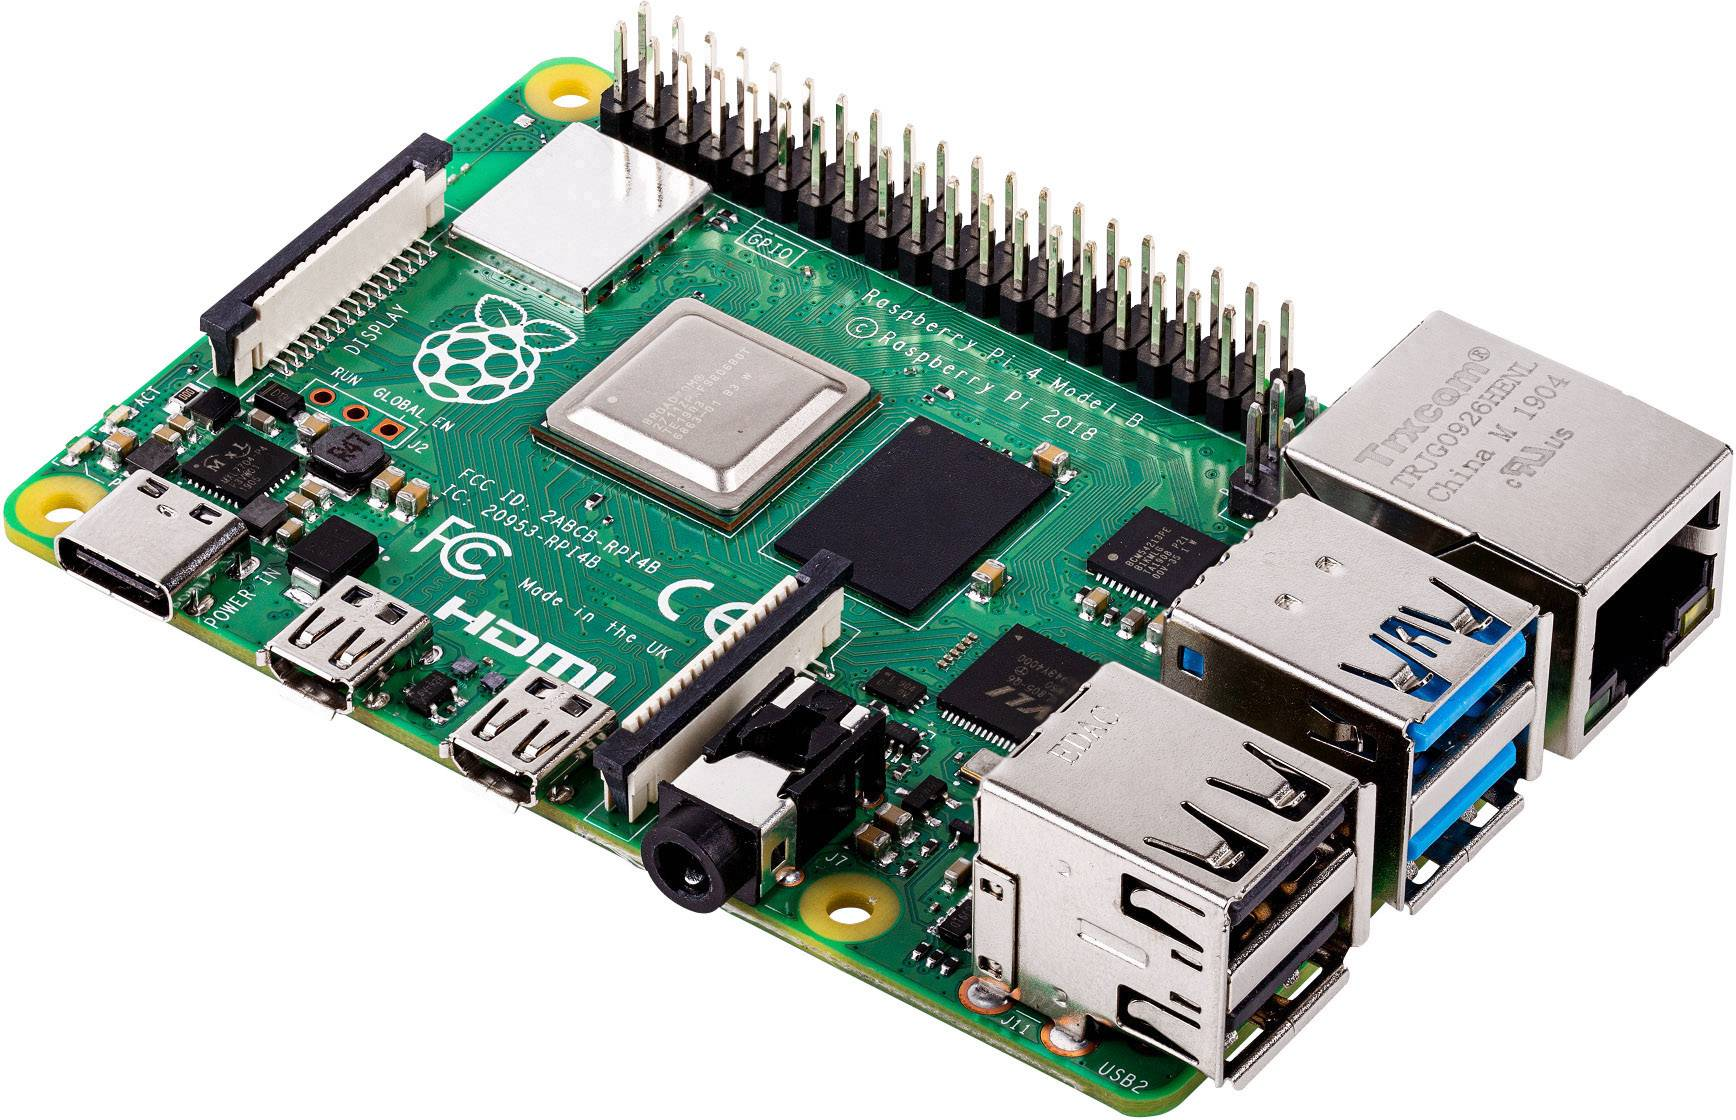
\includegraphics[height=3cm]{./01_Inhalte/07_RaspberryPi.jpg}
		\centering
		\caption{\acl{RasPi} 4}
	\end{figure}
\end{comment}

\subsection{\acl{RasPi} - Setup}
Um die Betriebssoftware auf die microSD-Karte zu schreiben, verwende ich Raspberry Pi Imager (Abbildung \ref{fig:RaspberryPiImager}). Als Systemsoftware würde ich empfehlen, Raspberry Pi OS (64 Bit) zu verwenden. Jedoch kann selbstverständlich auch ein anderes Betriebssystem bzw. die Lite/Full-Version davon benützt werden.

\begin{minipage}{0.5\textwidth}
	\begin{figure}[H]
		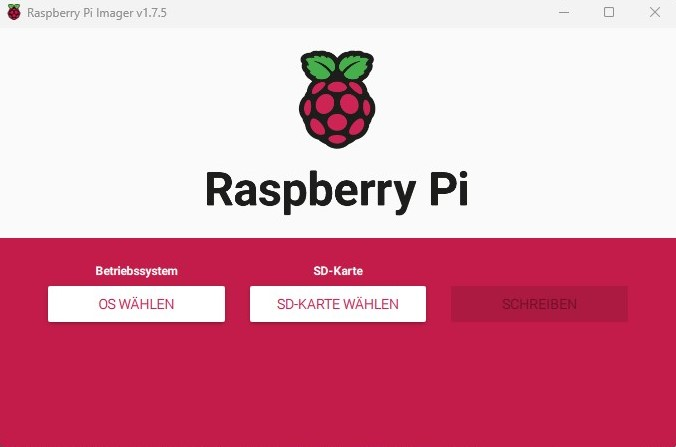
\includegraphics[height=5cm]{./01_Inhalte/08_Imager.jpg}
		\centering
		\caption{Raspberry Pi Imager}
		\label{fig:RaspberryPiImager}
	\end{figure}
\end{minipage}%
\begin{minipage}{0.5\textwidth}		
	\begin{figure}[H]
		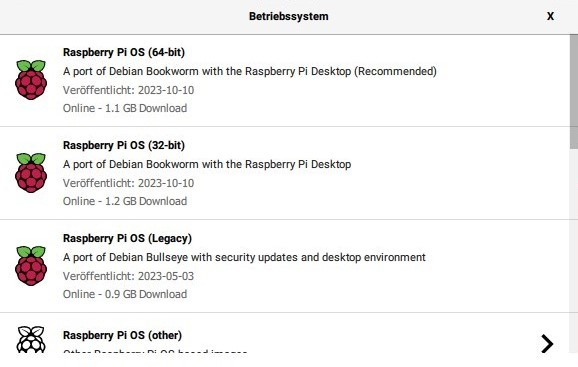
\includegraphics[height=5cm]{./01_Inhalte/08a_RaspberryPi_OS.jpg}
		\centering
		\caption{Raspberry Pi OS (64 Bit)}
		\label{fig:RaspberryPiOS}
	\end{figure}
\end{minipage}	
\\ \\
Nach Auswahl des Betriebssystems ist es ratsam noch unter den erweiterten Einstellung (Abbildung \ref{fig:ImagerOptionen}) einen Hostnamen zu vergeben und SSH zu aktivieren. Je nach Bedarf kann hier auch direkt eine WLAN-Verbindung eingerichtet werden. In diesem Fall werden für die SSH-Verbindung folgenden Zugangsdaten verwendet:


\begin{minipage}{0.5\textwidth}
	\begin{itemize}
		\item Benutzername: admin
		\item Passwort: Kennwort1
	\end{itemize}
\end{minipage}%
\begin{minipage}{0.5\textwidth}		
	\begin{figure}[H]
		\centering
		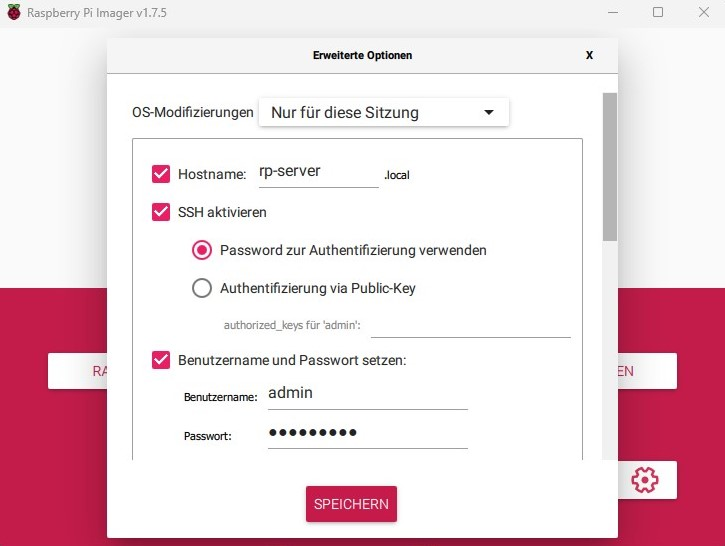
\includegraphics[width=6.8cm]{./01_Inhalte/08b_Imager_Optionen.jpg}
		\caption{Erweiterte Optionen}
		\label{fig:ImagerOptionen}
	\end{figure}
\end{minipage}	



Nach Abschluss des Schreibe- und Verifizierungsvorgangs kann die microSD-Karte entfernt und in den \ac{RasPi} eingesetzt werden. Sobald die IP-Adresse bekannt ist, ist es möglich, sich beispielsweise mit PuTTY über SSH mit dem \ac{RasPi} zu verbinden.

\begin{figure}[H]
	\centering
	\begin{subfigure}[t]{0.35\textwidth}
		\begin{adjustbox}{valign=c,center}
			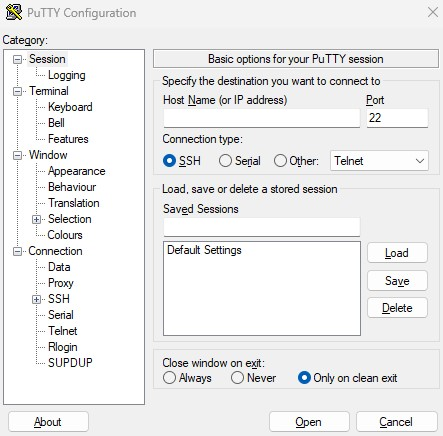
\includegraphics[width=\textwidth]{./01_Inhalte/08c_PuTTY.jpg}
		\end{adjustbox}
	\end{subfigure}
	\hfill
	\begin{subfigure}[t]{0.62\textwidth}
		\begin{adjustbox}{valign=c,center}
			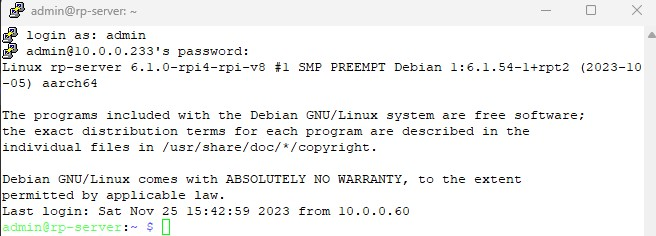
\includegraphics[width=\textwidth]{./01_Inhalte/08d_PuTTY.jpg}
		\end{adjustbox}
	\end{subfigure}
	\caption{PuTTY}
	\label{fig:PuTTY}
\end{figure}


\subsection{\ac{DBMS}}
Als \ac{DBMS} wird \textbf{MariadDB} verwendet. Zuerst sollte man die lokale Paketliste und alle installierten Softwarepakete aktualisieren. Falls man aufgefordert wird, fortzufahren, bestätige dies immer durch die Eingabe von ''Y''. Geben Sie die Befehle zudem immer einzeln ein.

\begin{Textfeld1}
	sudo apt update \\
	sudo apt upgrade
\end{Textfeld1}

Danach erfolgt die Installation des MariaDB-Servers durch Ausführen des folgenden Befehls:

\begin{Textfeld1}
	sudo apt install mariadb-server
\end{Textfeld1}

Nachdem die Installation abgeschlossen ist, führen wir die Grundkonfiguration mithilfe folgender Anweisung durch:

\begin{Textfeld1}
	sudo mysql\_secure\_installation
\end{Textfeld1}

Durch das Setup wie folgt durchgehen:

\begin{itemize}
	\item ''Enter current password for root'' = Bestätige mittels Enter-Taste (keine Eingabe).
	\item ''Switch to unix\_socket authentication?'' = n
	\item ''Change the root password?'' =  Y
	\begin{itemize}
		\item ''New password:'' = Kennwort1
		\item ''Re-enter new password:'' = Kennwort1
	\end{itemize}
	\item ''Remove anonymous users'' = Y
	\item ''Disallow root login remotely'' = Y
	\item ''Remove test database and access to it'' = Y
	\item ''Reload privilege tables now'' = Y
\end{itemize}

Um den Zugriff auf die \ac{DB} von anderen Rechnern zu ermöglichen, müssen wir noch den externen Zugriff aktivieren. Hierfür müssen wir folgendes File bearbeiten:

\begin{Textfeld1}
	sudo nano /etc/mysql/mariadb.conf.d/50-server.cnf
\end{Textfeld1}

Wir ändern die \textbf{bind-address} von 127.0.0.1 auf 0.0.0.0.

\begin{figure}[H]
	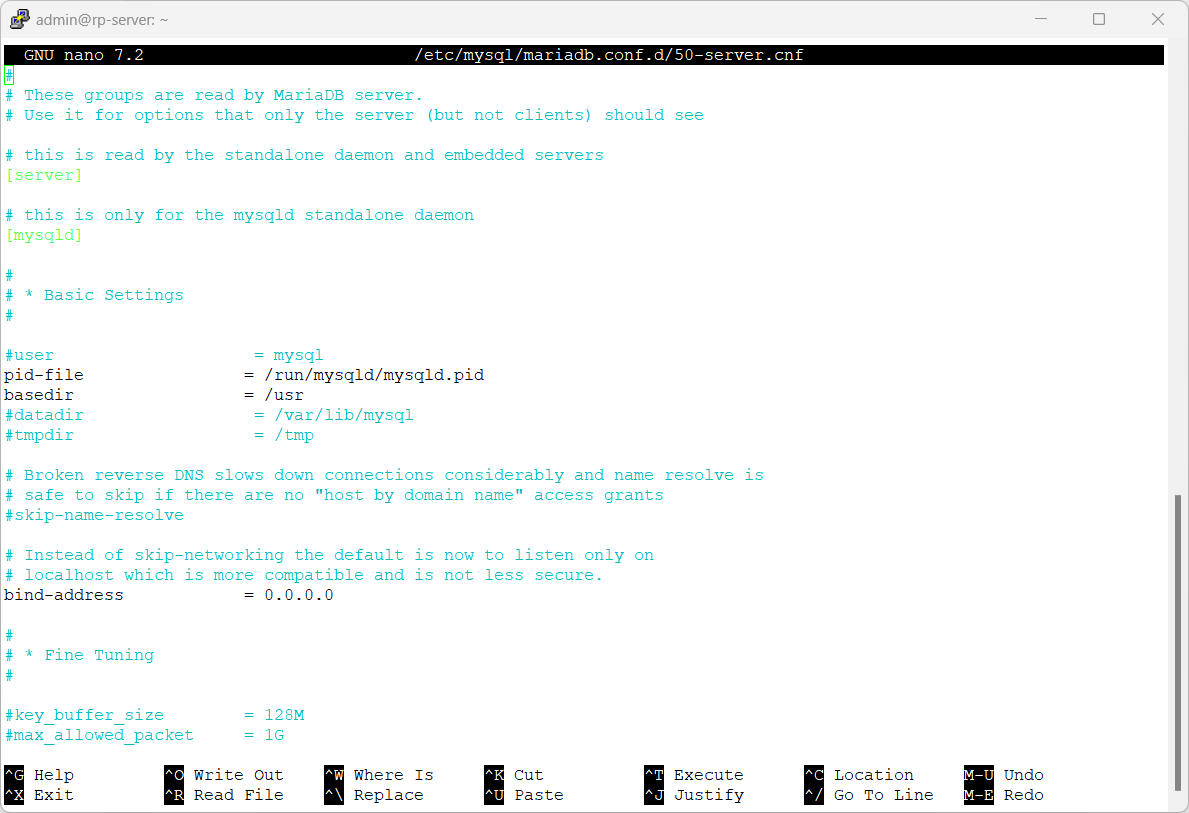
\includegraphics[scale=0.5]{./01_Inhalte/09_MariaDB_conf}
	\centering
	\caption{Externer Zugriff}
\end{figure}

Mit ''STR + O'' und dann ''Enter'' können wir die Änderungen speichern. Mittels der Tastenkombination ''STR + X'' verlassen wir danach den Editor.

\newpage
Im Anschluss müssen wir noch die Datenbank anlegen. Zu diesem Zweck verbinden wir uns mit dem Root-Account auf die \ac{DB}, in dem wir folgenden Befehl verwenden:

\begin{Textfeld1}
	sudo mysql -u root -p
\end{Textfeld1}

Daraufhin wird man aufgefordert das Passwort für den Root-User einzugeben, welches ''Kennwort1'' ist. Nun befinden wir uns in der MySQL-Shell, in welcher wir unsere SQL-Befehle ausführen können. Zuerst erstellen wir eine neue Datenbank mit folgender Anweisung:

\begin{Textfeld2}
	CREATE DATABASE Zeitmessung;
\end{Textfeld2}

Zusätzliche legen wir noch einen neuen Account an der nur Rechte über diese Datenbank besitzt.

\begin{itemize}
	\item Benutzername: mariadbclient
	\item Password: Kennwort1
\end{itemize}


Durch die Ausführung dieses Befehls wird der Benutzer erstellt:
\begin{Textfeld2}
	CREATE USER 'mariadbclient'@'\%' IDENTIFIED BY 'Kennwort1'; 
\end{Textfeld2}

Danach müssen wir diesem Benutzer noch Berechtigungen für die zuvor erstellte \ac{DB} erteilen:
\begin{Textfeld2}
	GRANT ALL PRIVILEGES ON Zeitmessung.* TO 'mariadbclient'@'\%'; 
\end{Textfeld2}

Zuletzt müssen wir noch die Berechtigungen neu laden:
\begin{Textfeld2}
	FLUSH PRIVILEGES;
\end{Textfeld2}

Um die MySQL-Shell zu verlassen und zur normalen Linux-Shell zurückzukehren, verwenden wir folgende Anweisung:

\begin{Textfeld2}
	exit;
\end{Textfeld2}

Es ist ratsam nach der Installation des Mariadb-Servers den \ac{RasPi} neu zu starten:
\begin{Textfeld1}
	sudo reboot
\end{Textfeld1}

Auf diese Weise haben wir erfolgreich das \ac{DBMS} installiert und müsse nun nur noch die benötigten Tabellen erstellten. Hierfür muss man lediglich die \ac{GUI} (Abschnitt \ref{sec:GUI}) einmalig starten und alle noch nicht vorhandenen Tabellen werden automatisch erzeugt. Dieser Schritt sollte jedoch erst nach Installation des MQTT-Brokers durchgeführt werden, um potenzielle Verbindungsfehler mit dem  Broker zu vermeiden.

\begin{figure}[H]
	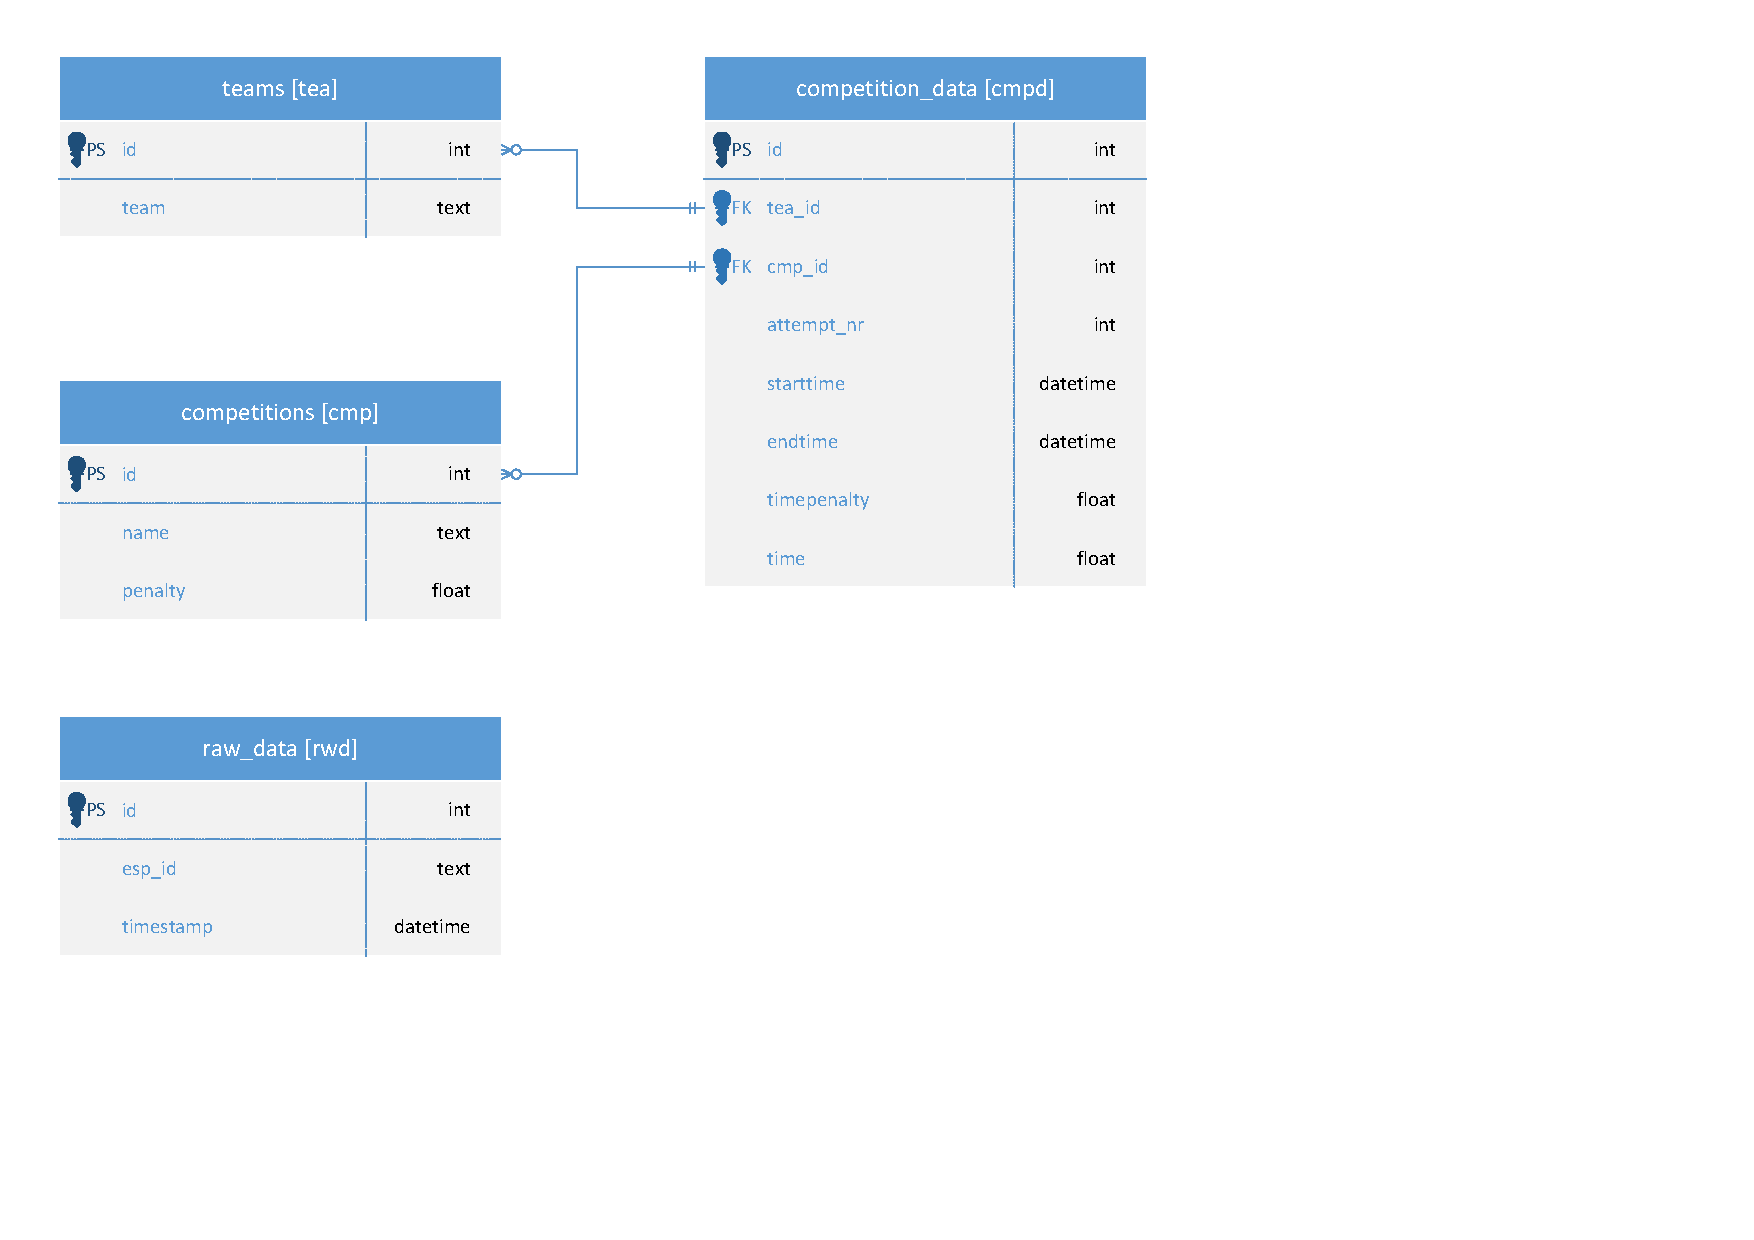
\includegraphics[width=0.65\textwidth]{./01_Inhalte/10_DB_Struktur.pdf}
	\centering
	\caption{\ac{DB}-Struktur}
\end{figure}


\subsubsection{PHPMyAdmin}
Zur leichteren Handhabung der MariaDB-Datenbank empfehle ich PHPMyAdmin zu installieren:
\begin{Textfeld1}
	sudo apt install phpmyadmin
\end{Textfeld1}
Falls man aufgefordert wird, fortzufahren, bestätige dies immer durch die Eingabe von ''Y''. Durch das Setup wie folgt durchgehen:
\begin{itemize}
	\item ''Web server to reconfigure automatically:'' = apache2 mit Leertaste auswählen und mit Enter bestätigen
	\item ''Configure database for phpmyadmin with dbconfig-common?'' = Yes mit Leertaste bestätigen
	\item ''MySQL application password for phpmyadmin:'' = ''Kennwort1'' mit Enter bestätigen
	\item ''Password confirmation:'' = ''Kennwort1'' mit Enter bestätigen
\end{itemize}
Somit wurde PHPMyAdmin erfolgreich installiert. Mittels der IP-Adresse des \ac{RasPi} und der Erweiterung ''/phpmyadmin'' kann lokal im Webbrowser auf die Anwendung zugegriffen werden (z.B.: 192.168.0.x/phpmyadmin). Als Benutzer würde ich empfehlen den Root-Account zu verwenden, da dieser Zugriffsrechte auf alle Datenbanken besitzt:
\begin{itemize}
	\item Benutzername: root
	\item Passwort: Kennwort1
\end{itemize} 


\subsection{MQTT Broker}
Zunächst installieren wir den MQTT-Broker. Wir verwenden in diesem Fall Mosquitto.
\begin{Textfeld1}
	sudo apt install mosquitto
\end{Textfeld1}

Anschließend stellen wir sicher das Mosquitto bei einem Neustart automatisch startet:
\begin{Textfeld1}
	sudo systemctl enable mosquitto
\end{Textfeld1}

Abschließend erstellen wir noch einen Benutzer für den MQTT-Broker:
\begin{itemize}
	\item Benutzername: mqttclient
	\item Password: Kennwort1
\end{itemize}
\begin{Textfeld1}
	sudo mosquitto\_passwd -c /etc/mosquitto/credentials mqttclient
\end{Textfeld1}

Daraufhin werden wir aufgefordert das Password einzugeben:
\begin{itemize}
	\item ''New password:'' = Kennwort1
	\item ''Re-enter new password:'' = Kennwort1
\end{itemize}

Hierdurch wird automatische eine Passwort-Datei erzeugt. Nun müssen wir Mosquitto noch konfigurieren:
\begin{Textfeld1}
	sudo nano /etc/mosquitto/conf.d/local.conf
\end{Textfeld1}

\newpage
In diese Konfigurations-Datei fügen wir noch folgende Zeilen ein:
\begin{figure}[H]
	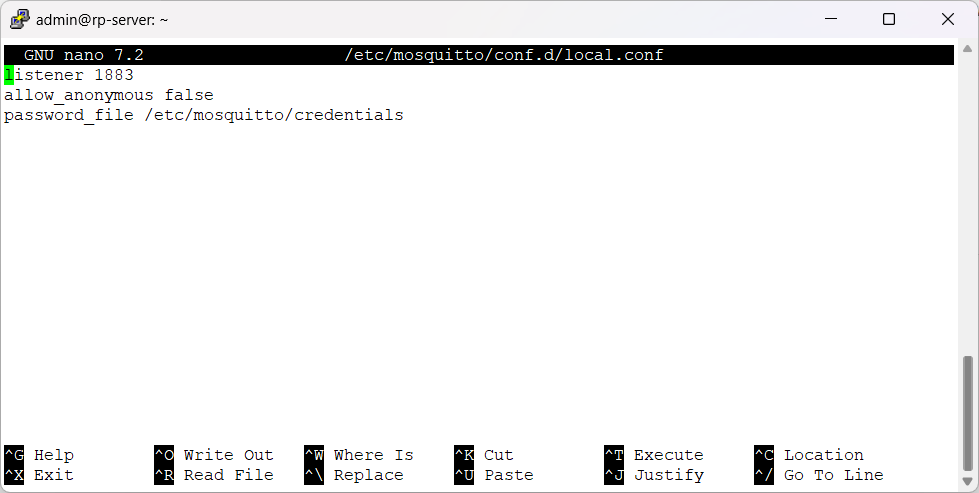
\includegraphics[width=0.9\textwidth]{./01_Inhalte/11_Mosquitto_conf}
	\centering
	\caption{Mosquitto Konfiguration}
\end{figure}

Mit ''STR + O'' und dann ''Enter'' können wir die Änderungen speichern. Mittels der Tastenkombination ''STR + X'' verlassen wir danach den Editor. Damit die eben erstellte Konfiguration wirksam wird starten wir Mosquitto neu:
\begin{Textfeld1}
	sudo systemctl restart mosquitto
\end{Textfeld1}

Somit haben wir den MQTT-Broker erfolgreich installiert und konfiguriert.

\begin{comment}
	\subsection{Webserver \& Services}
	Für die übersichtliche Darstellung der Ergebnisse der einzelnen Teams bzw. Challenges sowie des gesamten Bewerbs wurde ein Webserver konstruiert. Damit dieser funktioniert, müssen einige Dateien auf den \ac{RasPi} kopiert und Services hierfür aktiviert werden. Darüber hinaus verfügt das Service über eine Anwendung, welche alle Zeitstempel der Lichtschranke erfasst und speichert, unabhängig davon, ob sie verwendet werden. Hierfür muss der Ordner \textbf{01\_RP-Zeitmessung} auf das Homeverzeichnis des Benutzers ''admin'' (/home/admin) kopieren werden. Hierfür würde ich \textbf{WinSCP} empfehlen. Wird ein anderer Pfad gewünscht bzw. verwendet, muss man in den Dateien \textbf{startup\_script.sh} und \textbf{webserver.service}, welche sich im Verzeichnis \textbf{01\_RP-Zeitmessung} befinden, den Pfad anpassen, um den fehlerfreien Betrieb sicherzustellen. Bevor man jedoch den das Service aktiviert, muss man noch die Benutzerdaten im Python-Programm \textbf{app.py} im Verzeichnis \textbf{01\_RP-Zeitmessung} anpassen. Hierfür ist es ratsam, dies direkt in Visual Studio Code zu erledigen, bevor man den Ordner auf den \ac{RasPi} kopiert.
	\begin{lstlisting}[language=Python]
		# Database configuration
		DB_USER = "mariadbclient"       
		DB_PASSWORD = "Kennwort1"       
	\end{lstlisting}
	
	Zusätzlich muss man auch noch die Benutzerdaten im Programm \textbf{raw\_esp.py} im Ordner \textbf{01\_RP-Zeitmessung} modifizieren:
	\begin{lstlisting}[language=Python]
		# MQTT configuration
		MQTT_USER = "mqttclient"        
		MQTT_PASSWORD = "Kennwort1"    
		
		# Database configuration
		DB_USER = "mariadbclient"       
		DB_PASSWORD = "Kennwort1"     
	\end{lstlisting}
	
	Daraufhin kopieren wir mittels WinSCP den Ordner \textbf{01\_RP-Zeitmessung} auf den \ac{RasPi} in das Verzeichnis \textbf{/home/admin}. 
	\begin{figure}[H]
		\centering
		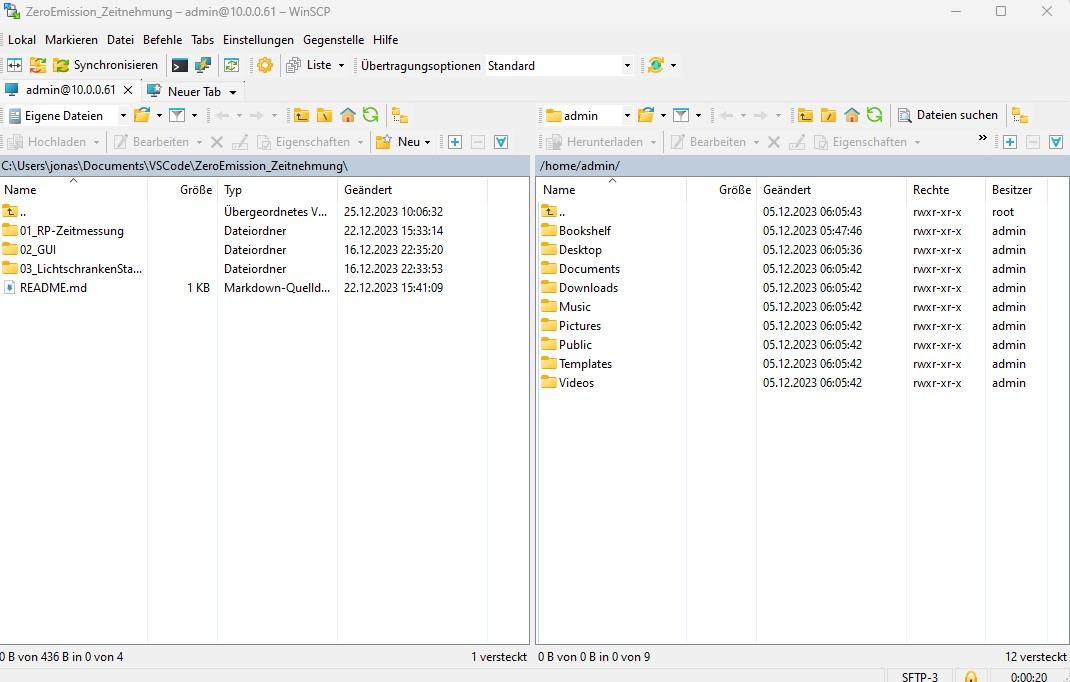
\includegraphics[width=0.85\textwidth]{./01_Inhalte/12_WinSCP}
		\caption{WinSCP}
	\end{figure}
	
	Danach müssen wir noch die Service-Datei in den richtigen Ordner verschieben.
	\begin{Textfeld1}
		sudo mv /home/admin/01\_RP-Zeitmessung/webserver.service /etc/systemd/system
	\end{Textfeld1}
	
	Anschließend müssen wir noch Ausführungsrechte rekursiv für das gesamte Verzeichnis erteilen:
	\begin{Textfeld1}
		chmod -R +x /home/admin/01\_RP-Zeitmessung
	\end{Textfeld1}
	
	Nachher laden wir mit dem folgenden Befehl den Systemd-Deamon neu :
	\begin{Textfeld1}
		sudo systemctl daemon-reload
	\end{Textfeld1}
	
	Als Nächstes starten wir das Service und aktivieren den automatischen Start bei Systemstart:
	\begin{Textfeld1}
		sudo systemctl start webserver \\
		sudo systemctl enable webserver
	\end{Textfeld1}
	
	Somit wurde der Webserver erfolgreich aktiviert. Man kann nun auf die Anwendung zugreifen, indem man die IP-Adresse des \ac{RasPi} und die Erweiterung '':5000'' in seinem Webbrowser eingibt. Zum Beispiel: \textbf{''192.168.0.x:5000''}.
\end{comment}


\subsection{Webserver \& Services}
Für die übersichtliche Darstellung der Ergebnisse der einzelnen Teams bzw. Challenges sowie des gesamten Bewerbs wurde ein Webserver konstruiert. Damit dieser funktioniert, müssen einige Dateien auf den \ac{RasPi} kopiert und der Apache2-Webserver hierfür konfiguriert werden. Darüber hinaus verfügt das Service über eine Anwendung, welche alle Zeitstempel der Lichtschranken erfasst und speichert, unabhängig davon, ob sie verwendet werden. Hierfür muss der Ordner \textbf{01\_RP-Zeitmessung} in das Verzeichnis \textbf{/var/www} kopieren werden. Hierfür würde ich \textbf{WinSCP} empfehlen. Bevor man jedoch den den Ordner auf den \ac{RasPi} kopiert, muss man noch die Benutzerdaten im Python-Programm \textbf{app.py} im Verzeichnis \textbf{01\_RP-Zeitmessung} anpassen. 
\newpage
Hierfür ist es ratsam, dies direkt in Visual Studio Code zu erledigen.

\begin{lstlisting}[language=Python]
	# MQTT configuration
	MQTT_USER = "mqttclient"        
	MQTT_PASSWORD = "Kennwort1"    
	
	# Database configuration
	DB_USER = "mariadbclient"       
	DB_PASSWORD = "Kennwort1"     
\end{lstlisting}

Danach kann man mit WinSCP den Ordner \textbf{01\_RP-Zeitmessung} auf den \ac{RasPi} ins Verzeichnis \textbf{''/home/admin''} kopieren, da dem Benutzer ''admin'' die Rechte fehlen für das Verzeichnis \textbf{''/var/www''}. Dies kann man direkt mit ''Drag and Drop'' durchführen.
\begin{figure}[H]
	\centering
	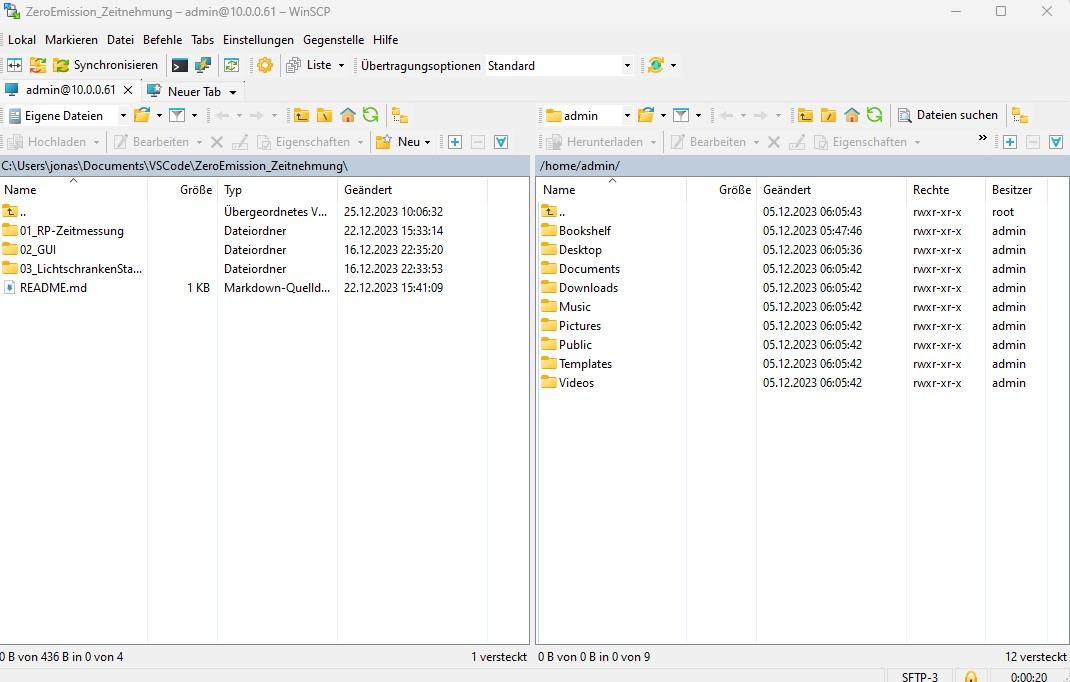
\includegraphics[width=0.85\textwidth]{./01_Inhalte/12_WinSCP}
	\caption{WinSCP}
\end{figure}

Folglich verschieben wir den Ordner mit Root-Rechten in das richtige Verzeichnis und ändern die Gruppenzugehörigkeit des Ordners. Die Befehle immer einzeln eingeben.
\begin{Textfeld1}
	sudo mv /home/admin/01\_RP-Zeitmessung /var/www \\
	sudo chown -R admin:www-data /var/www/01\_RP-Zeitmessung
\end{Textfeld1}

Anschließend muss man die Serverkonfigurations-Datei noch in das richtige Verzeichnis verschieben.
\begin{Textfeld1}
	sudo mv /var/www/01\_RP-Zeitmessung/webserver.conf /etc/apache2/sites-available
\end{Textfeld1}

Zudem muss man \textbf{mod\_wsgi} installieren und aktivieren:
\begin{Textfeld1}
	sudo apt install libapache2-mod-wsgi-py3 \\
	sudo a2enmod wsgi
\end{Textfeld1}

Darauf deaktivieren wir die Standartkonfiguration und aktivieren unsere Konfiguration:
\begin{Textfeld1}
	sudo a2dissite 000-default \\
	sudo a2ensite webserver
\end{Textfeld1}

Im Anschluss starten wir den Apache2-Server neu:
\begin{Textfeld1}
	sudo systemctl restart apache2
\end{Textfeld1}


\subsection{Implementierungsschritte}
Darüber hinaus ist es notwendig, die Teams und Herausforderungen manuell einzutragen. Dies kann auf zwei Arten erfolgen: entweder über phpMyAdmin für eine benutzerfreundliche Oberfläche oder direkt im Terminal. Um die Daten im Terminal einzufügen, beginnt man zunächst mit der Verbindung zur Datenbank:

\begin{Textfeld1}
	sudo mysql -u root -p
\end{Textfeld1}
Daraufhin wird man aufgefordert das Passwort für den Root-User einzugeben, welches ''Kennwort1'' ist. Danach wählen wir die Datenbank aus:

\begin{Textfeld2}
	USE Zeitmessung;
\end{Textfeld2}

Danach können wir schon die Teams eintragen:

\begin{Textfeld2}
	INSERT INTO teams (name) VALUES ('Team 1'), ('Team 2'), ('Team 3');
\end{Textfeld2}

Beziehungsweise die Challenges:
\begin{Textfeld2}
	INSERT INTO challenges (name,penalty) VALUES ('Challenge 1', 1.0), ('Challenge 2', 2.0);
\end{Textfeld2}

Mit folgenden Befehl kann man die MySQL-Shell verlassen:
\begin{Textfeld2}
	exit;
\end{Textfeld2}

Des Weiteren empfehle ich für den \ac{RasPi} eine statische IP-Adresse zu vergeben, welche im \ac{DHCP}-Server eingetragen werden muss.

\subsection{Allgemeine Befehle}
Zum Herunterfahren des \ac{RasPi} kann man diesen Befehl verwenden:
\begin{Textfeld1}
	sudo shutdown -P now
\end{Textfeld1}

Wenn ma überprüfen möchte, ob ein gewisses Service (z.B. MariaDB, Mosquitto) läuft, kann dies mit folgender Anweisung erfolgen:
\begin{Textfeld1}
	sudo systemctl status service\_name
\end{Textfeld1}

Möchte man ein Service stoppen bzw. starten, wird dieser Befehl verwendet:
\begin{Textfeld1}
	sudo systemctl stop service\_name \\
	sudo systemctl start service\_name
\end{Textfeld1}

Um das Service automatische bei Systemstart zu starten bzw. diesen Vorgang zu deaktivieren verwendet man:
\begin{Textfeld1}
	sudo systemctl enable service\_name \\
	sudo systemctl disable service\_name
\end{Textfeld1}


\newpage


\section{Lichtschranken-Station}
Hier wird die grundlegende Funktionsweise, sowie die verwendeten Bauteile der Lichtschranken-Station erklärt.

\subsection{Bauteile}
In der nachfolgenden Erklärung werden die verschiedenen Bauelemente, welche bei der Lichtschranken-Station verwendet werden, im Detail beschrieben.

\subsubsection{Lichtschranke}
\label{sec:Lichtschranke}
Als Lichtschranke kommt die Reflexlichtschranke \textbf{Sick WL9-2P330S14 }zum Einsatz. Einige Spezifikationen sind:

\begin{minipage}{0.6\textwidth}
	\begin{itemize}
		\item Versorgungsspannung: 10V DC - 30V DC
		\item Stromverbrauch: 20mA
		\item Reichweite: 4m
		\item Reaktionszeit: < 624µs
		\item Schaltausgang: PNP
	\end{itemize}
\end{minipage}%
\begin{minipage}{0.4\textwidth}		
	\begin{figure}[H]
		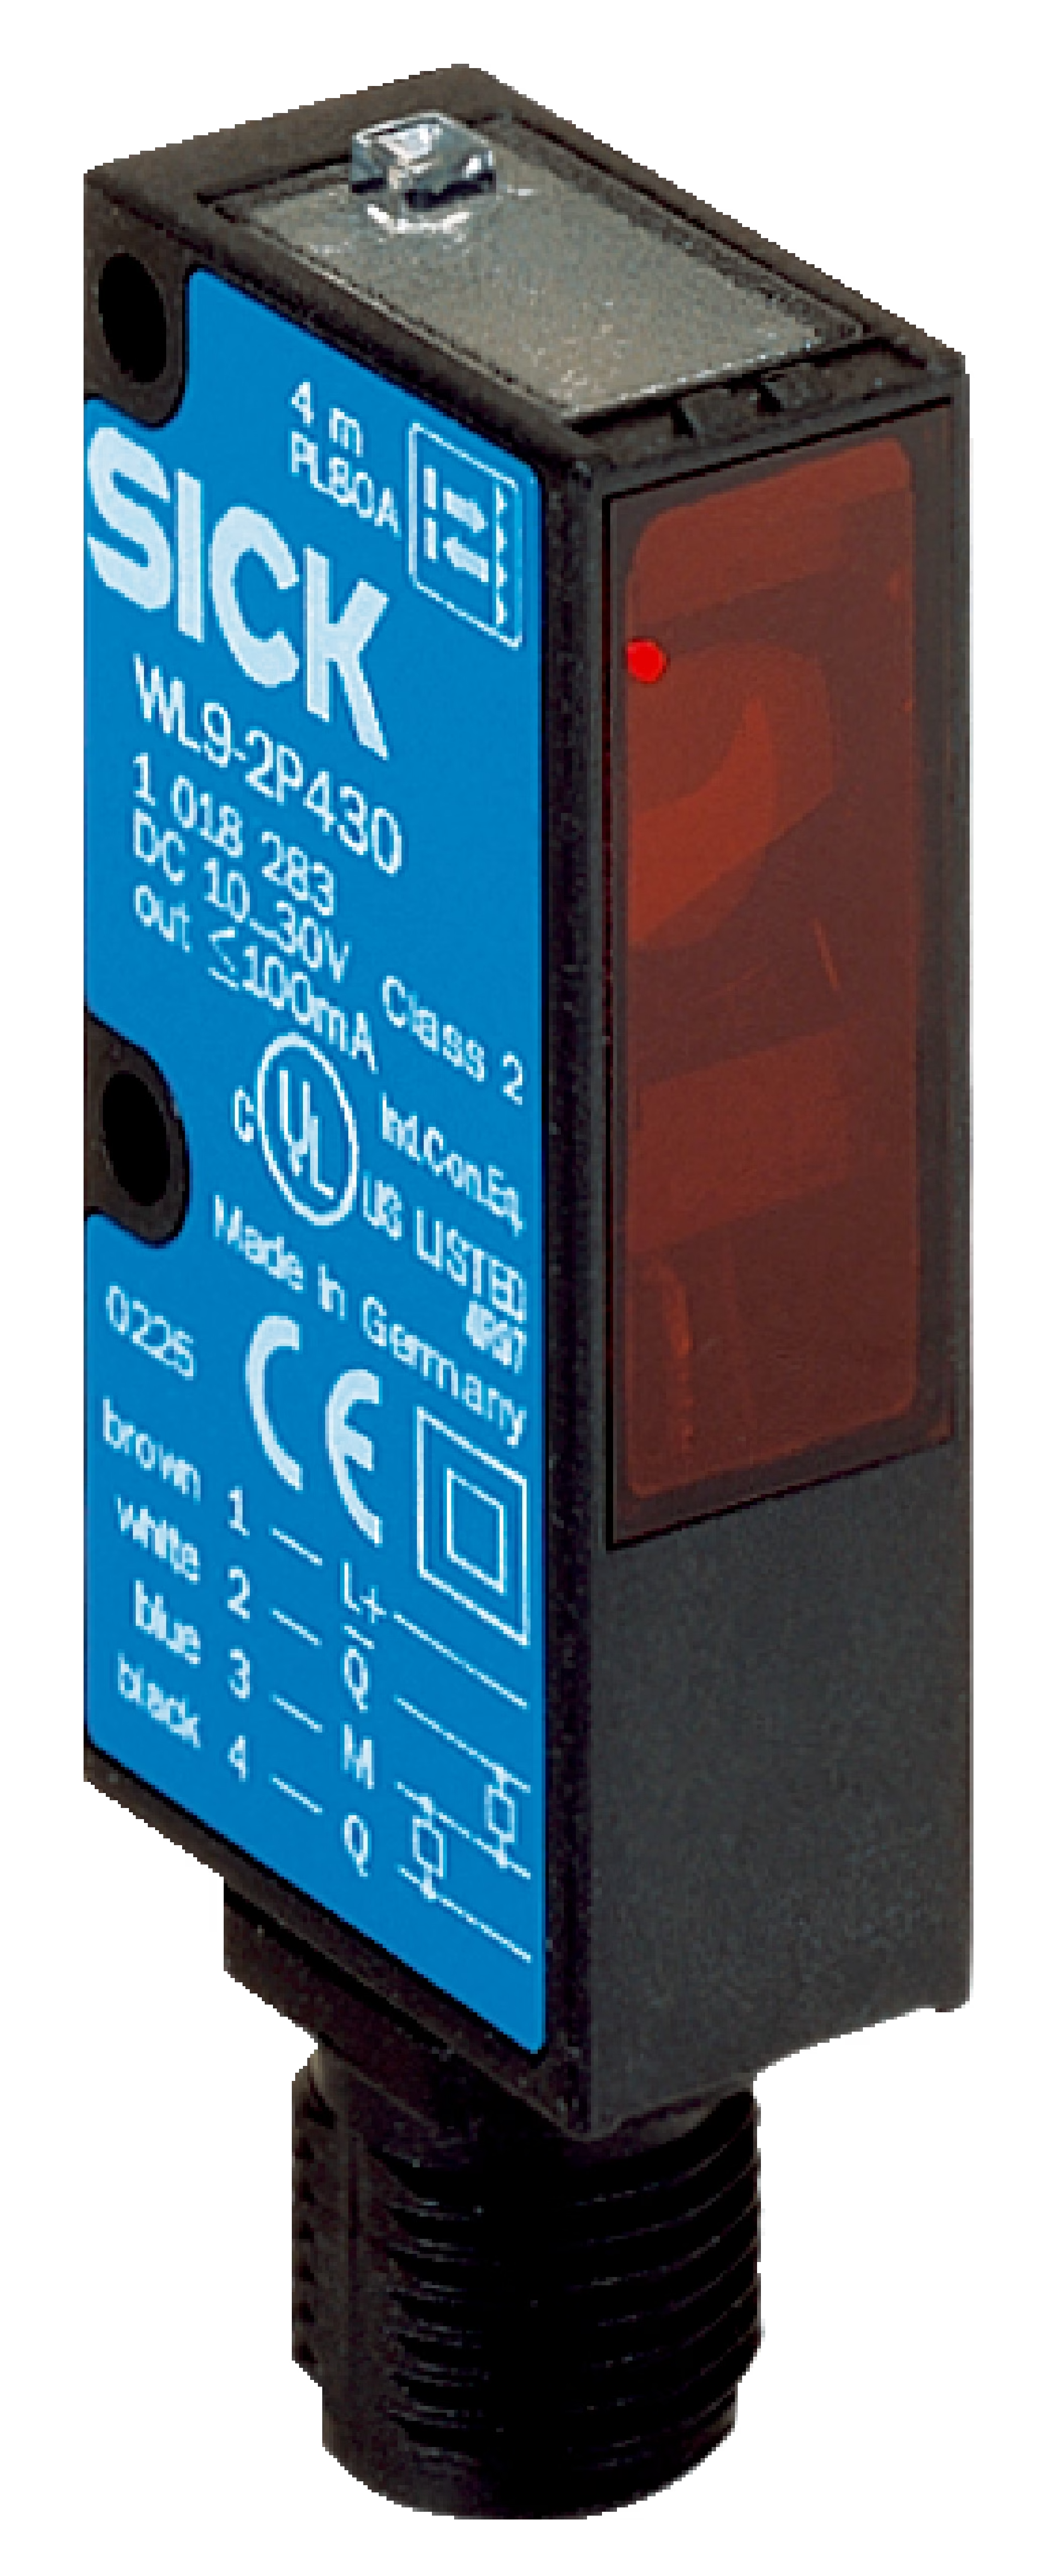
\includegraphics[scale=0.05]{./01_Inhalte/01_Lichtschranke.pdf}	
		\centering
		\caption{Reflexlichtschranke}
		\label{fig:Lichtschranke}
	\end{figure}
\end{minipage}	
\\ \\
Ist diese nicht ausgelöst, ist der Ausgang mit der positiven Eingangsspannung verbunden. Löst die Lichtschranke aus wird der Ausgang auf Masse gezogen. Da der Spannungsbereich der Reflexlichtschranke nicht mit dem des ESP32 übereinstimmt, muss der Ausgang an den Spannungsbereich des ESP32 angepasst werden. Dies wird durch einen Pegelwandler (Level Shifter) erzielt. Weiters ist zu beachten, dass die maximale Reichweite von 4m nur in Verbindung mit dem Reflektor \textbf{PL80A} (Abbildung \ref{fig:PL80A}) erzielt werden kann. Dieser besitzt über eine Reflexionsfläche mit den Maßen 80mm x 80mm.

\begin{figure}[H]
	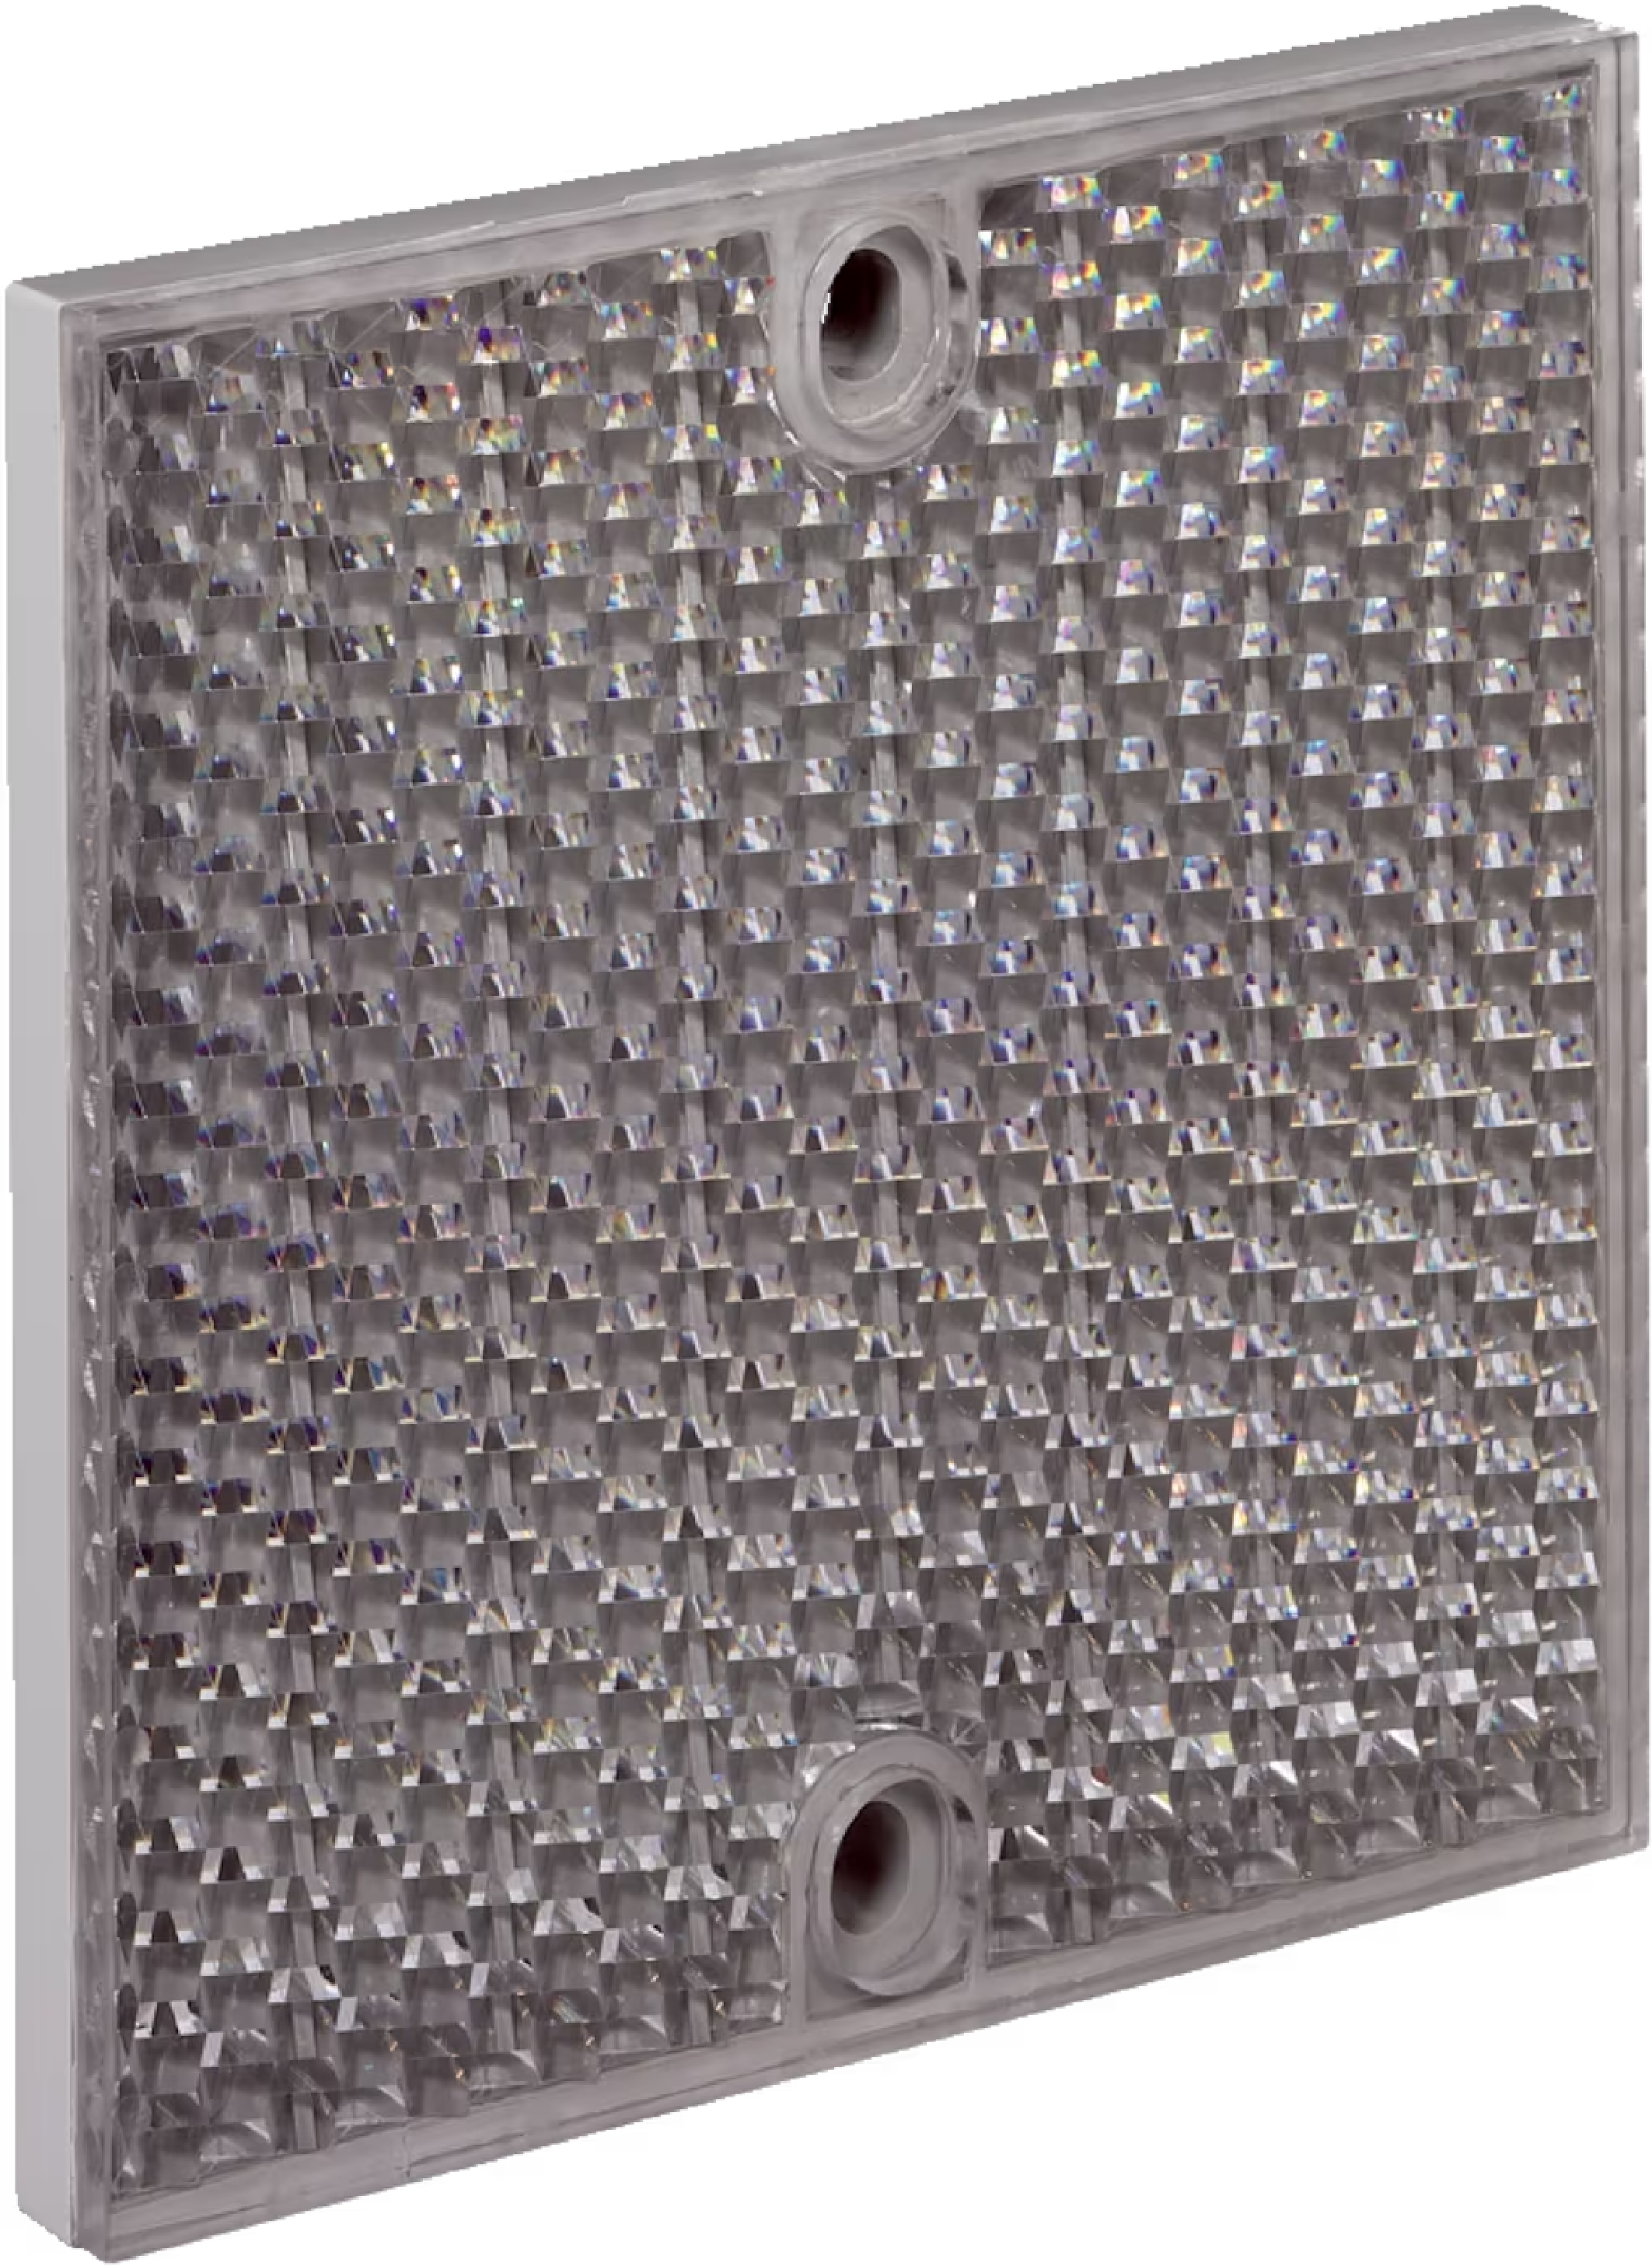
\includegraphics[height=4.6cm]{./01_Inhalte/01a_PL80A.pdf}	
	\centering
	\caption{PL80A-Reflektor}
	\label{fig:PL80A}
\end{figure}


\subsubsection{\ac{µC}}
Als \textbf{\ac{µC}} wird hier der \textbf{ESP32-S2-LCD} der Firma Waveshare verwendet. Standardmäßig ist bereits ein Display verbaut, das später dazu verwendet wird, die Zeitstempel der letzten Auslösung der Lichtschranke anzuzeigen.

\begin{minipage}{0.6\textwidth}
	\begin{itemize}
		\item Xtensa single-core 32-bit LX7 Mikroprozessor
		\item 2.4 GHz WiFi Keramik-Antenne
		\item 0.96-Zoll LCD Display
	\end{itemize}
\end{minipage}%
\begin{minipage}{0.4\textwidth}		
	\begin{figure}[H]
		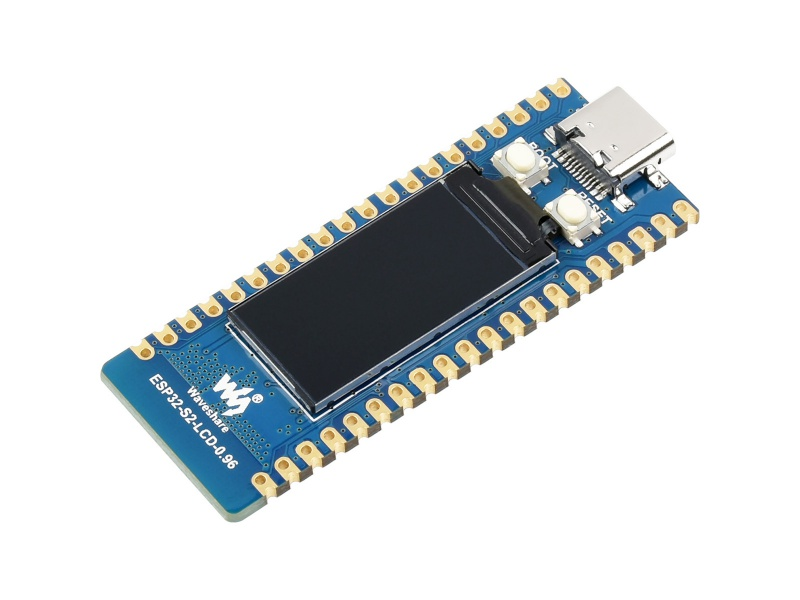
\includegraphics[scale=0.2]{./01_Inhalte/02_ESP32-S2-LCD.jpg}	
		\centering
		\caption{ESP32-S2-LCD}
		\label{fig:ESP32-S2-LCD}
	\end{figure}
\end{minipage}	

\begin{figure}[H]
	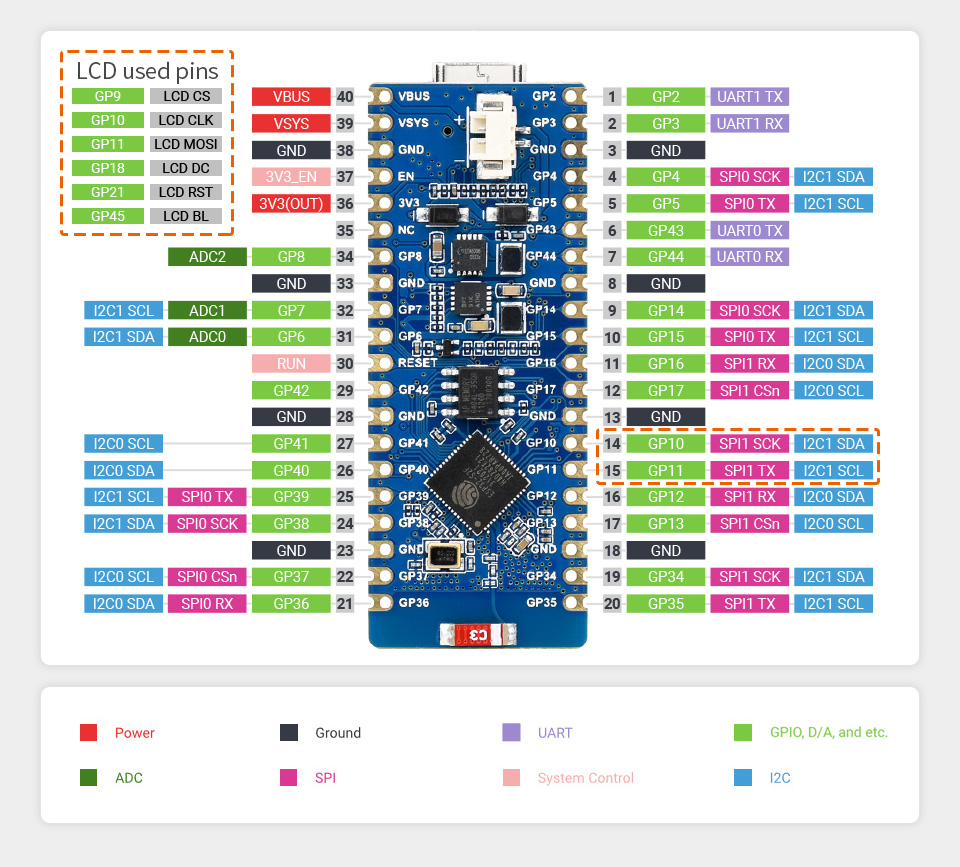
\includegraphics[width=\textwidth]{./01_Inhalte/02a_ESP32-S2-LCD_Pinout.jpg}	
	\centering
	\caption{ESP32-S2-LCD Pinout}
	\label{fig:ESP32-S2-LCD_Pinout}
\end{figure}



\subsubsection{GPS-Modul}
Zur Synchronisation der \textbf{\ac{RTC}} der \acl{µC} wird das GPS Modul \textbf{U-Blox Neo-6MV2} verwendet. Hierdurch wird gewährleistet, dass alle ESP32 exakt dieselbe Zeit bekommen.

\begin{minipage}{0.65\textwidth}
	\begin{itemize}
		\item Versorgungsspannung: 3V DC - 5V DC
		\item Maximaler E / A-Logikpegel: 3.6V
		\item Stromverbrauch: 40mA
		\item Kommunikationsinterface: UART TTL, 9600bps
		\item Zeitgenauigkeit: 1µs
		\item Betriebstemperatur: -40°C - +80°C
	\end{itemize}
\end{minipage}%
\begin{minipage}{0.35\textwidth}		
	\begin{figure}[H]
		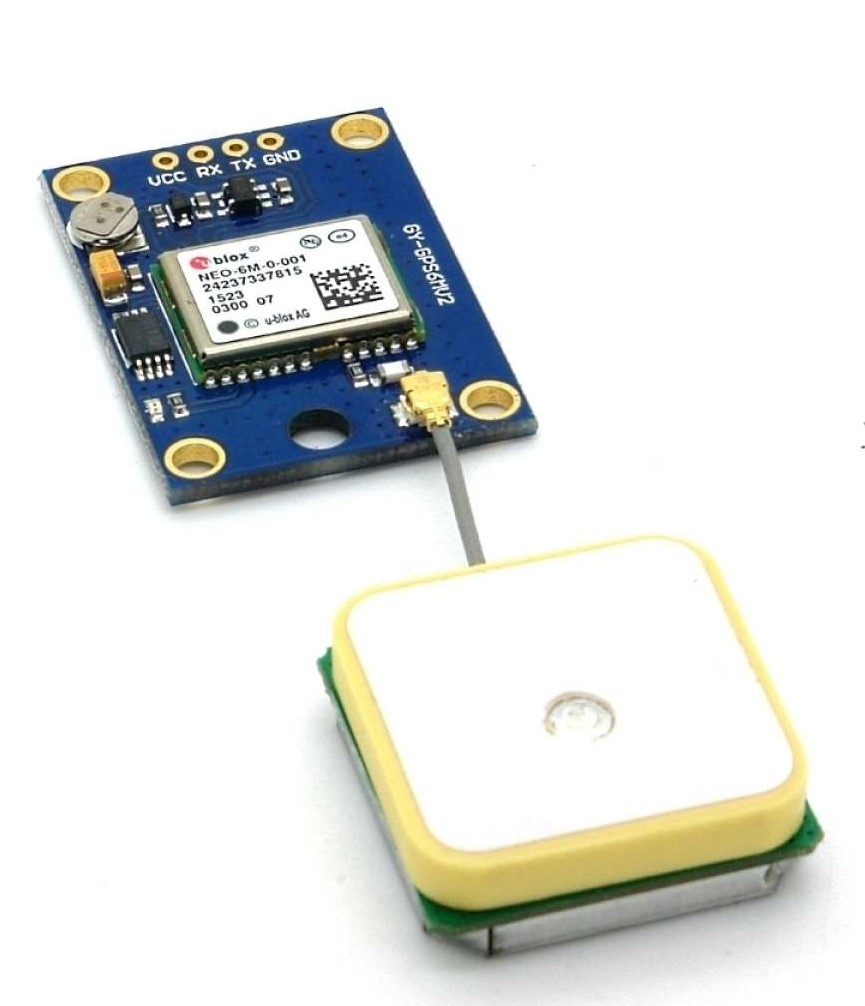
\includegraphics[scale=0.2]{./01_Inhalte/03_GPS-Modul.jpg}	
		\centering
		\caption{U-Box Neo-6M}
		\label{fig:GPS-Modul}
	\end{figure}
\end{minipage}	



\subsubsection{Stromversorgung}
Als Stromversorgung für die Station wird ein handelsüblicher Makita Akku verwendet.

\begin{minipage}{0.6\textwidth}
	\begin{itemize}
		\item Nennspannung: 18V
		\item Entladeschlussspannung: 15V
		\item Ladespannung: 21V 
		\item Kapazität: 108Wh
		\item Akkutyp: Li-ion
	\end{itemize}
\end{minipage}%
\begin{minipage}{0.4\textwidth}		
	\begin{figure}[H]
		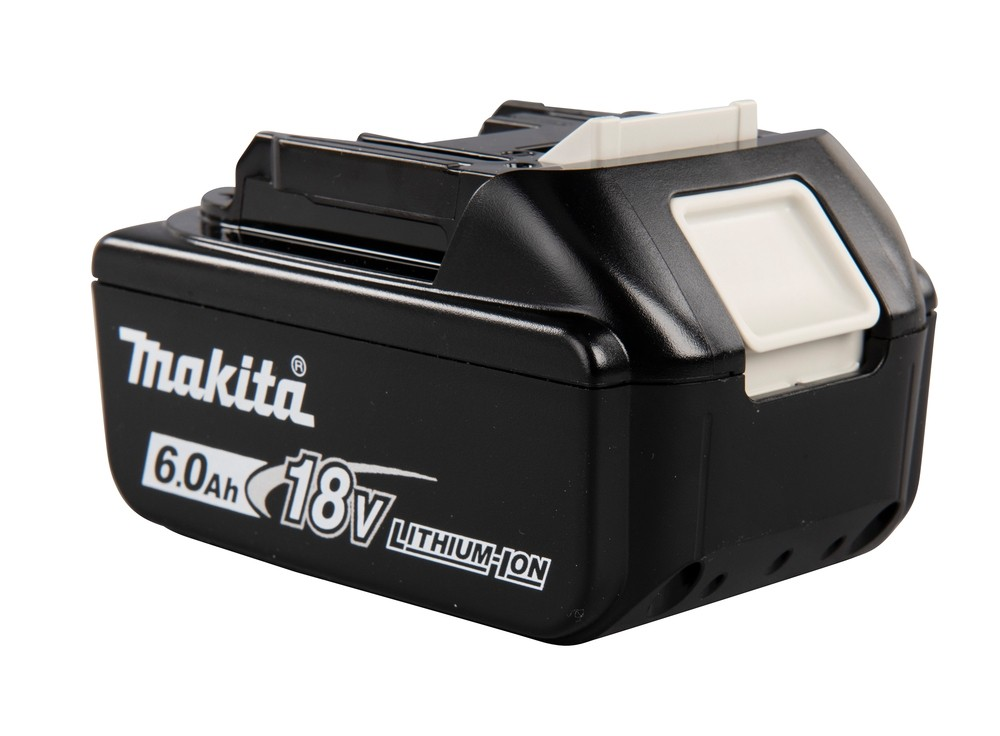
\includegraphics[scale=0.2]{./01_Inhalte/04_Makita-Akku.jpg}	
		\centering
		\caption{Makita-Akku}
		\label{fig:Makita-Akku}
	\end{figure}
\end{minipage}	

\subsubsection{DC-DC Wandler}
Für die Versorgung des ESP32-S2 wird eine Spannung von rund 5V benötigt. Diese wird durch den Buck-Schaltregler \textbf{OKI-78SR-5/1.5-W36-C} der Firma Murata PS bereitgestellt.


\begin{minipage}{0.45\textwidth}
	\begin{itemize}
		\item Eingangspannung: 7-36V DC
		\item Ausgangsspannung: 5V
		\item Maximaler Ausgangsstrom: 1,5A
	\end{itemize}
\end{minipage}%
\begin{minipage}{0.55\textwidth}		
	\begin{figure}[H]
		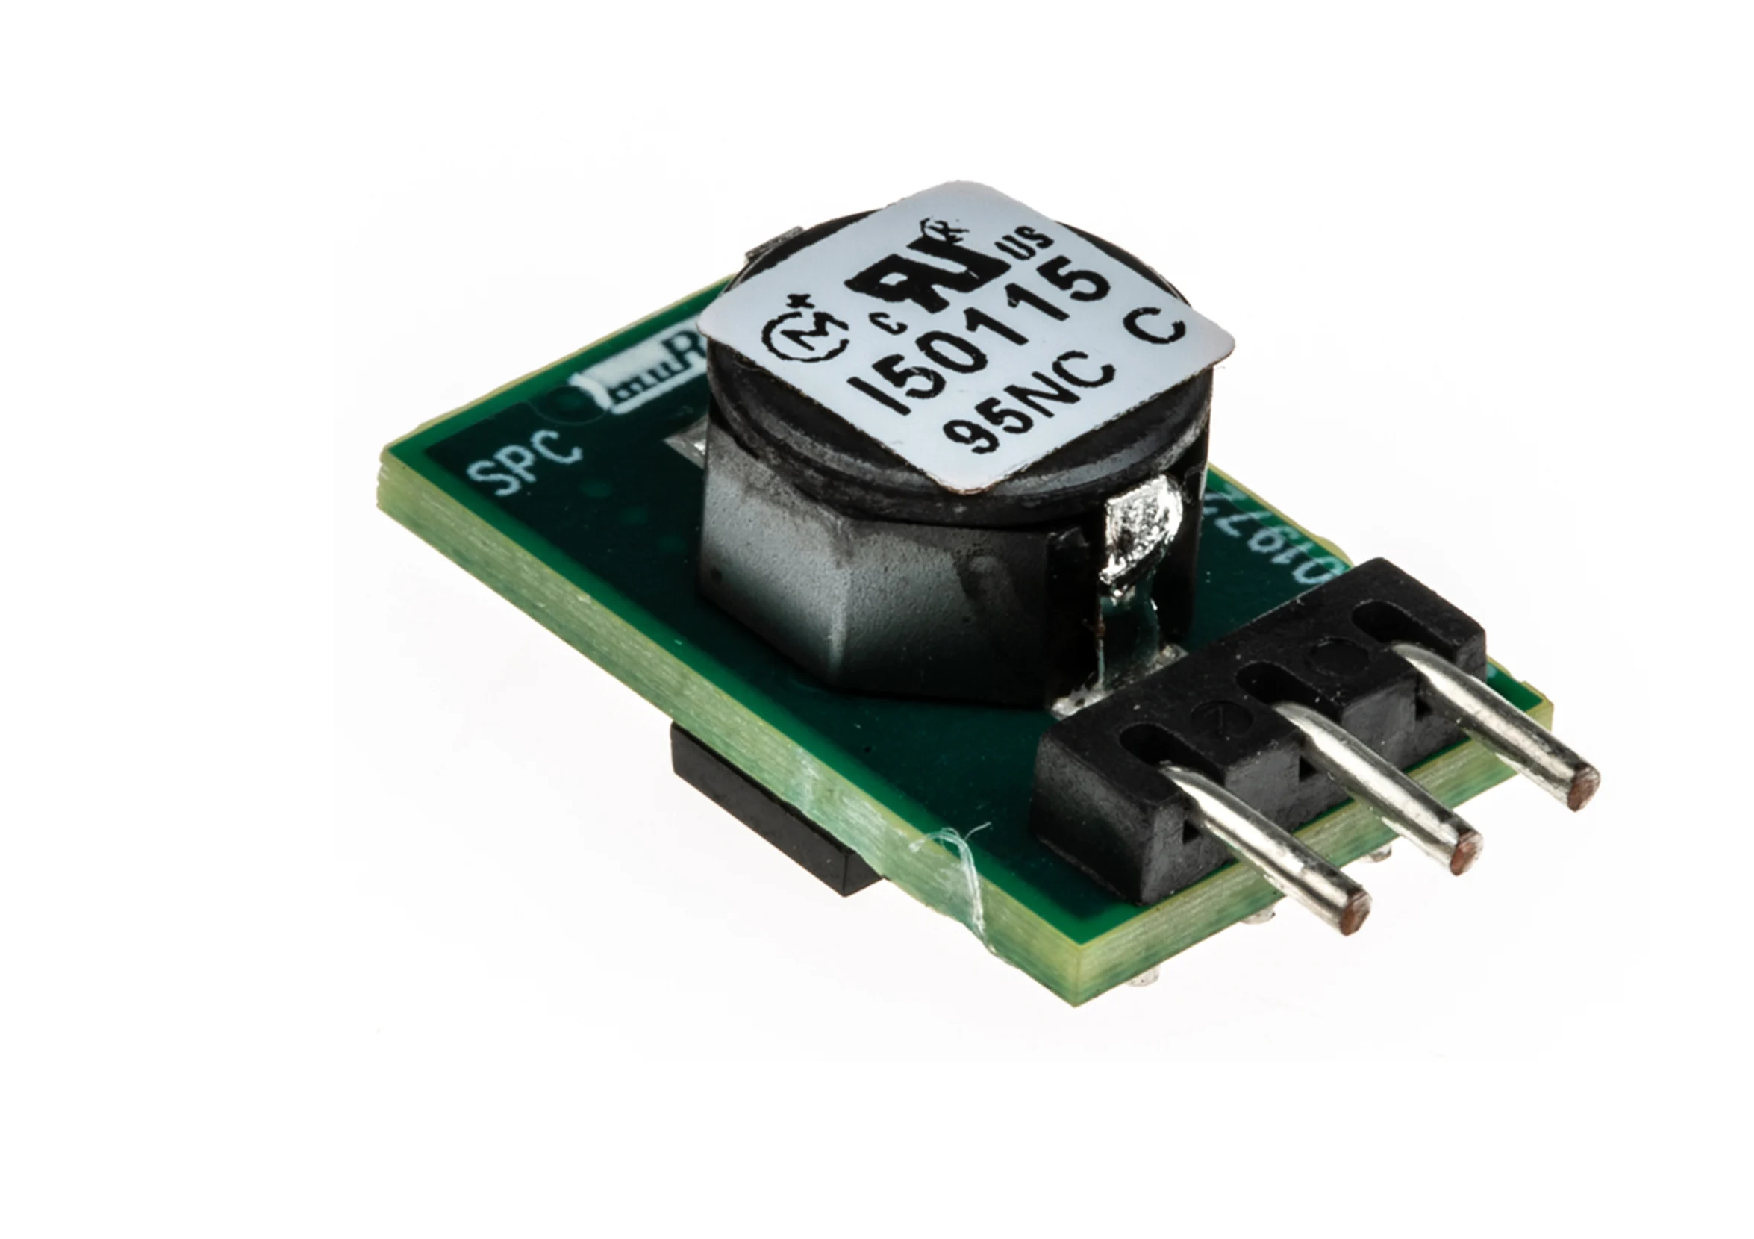
\includegraphics[scale=0.2]{./01_Inhalte/05_DC-DC.pdf}	
		\centering
		\caption{Murata PS OKI-78SR-5/1.5-W36-C}
		\label{fig:DC-DC}
	\end{figure}
\end{minipage}	


\subsubsection{Schaltplan}
Die vorher genannten Bauelemente werden wie in Abbildung \ref{fig:Lichtschranke-Schaltplan} dargestellt verschalten. Hinzu kommt noch der in Kapitel \ref{sec:Lichtschranke} genannte Pegelwandler mittels eines NPN-Transistors. Löst die Lichtschranke aus liegt an ihrem Ausgang (Q) eine Pegel von 0V an. Durch das Level Shifting liegt dadurch am GPIO15-Pin des ESP32 ein Spannungspegel von 3,3V an.

\begin{figure}[H]
	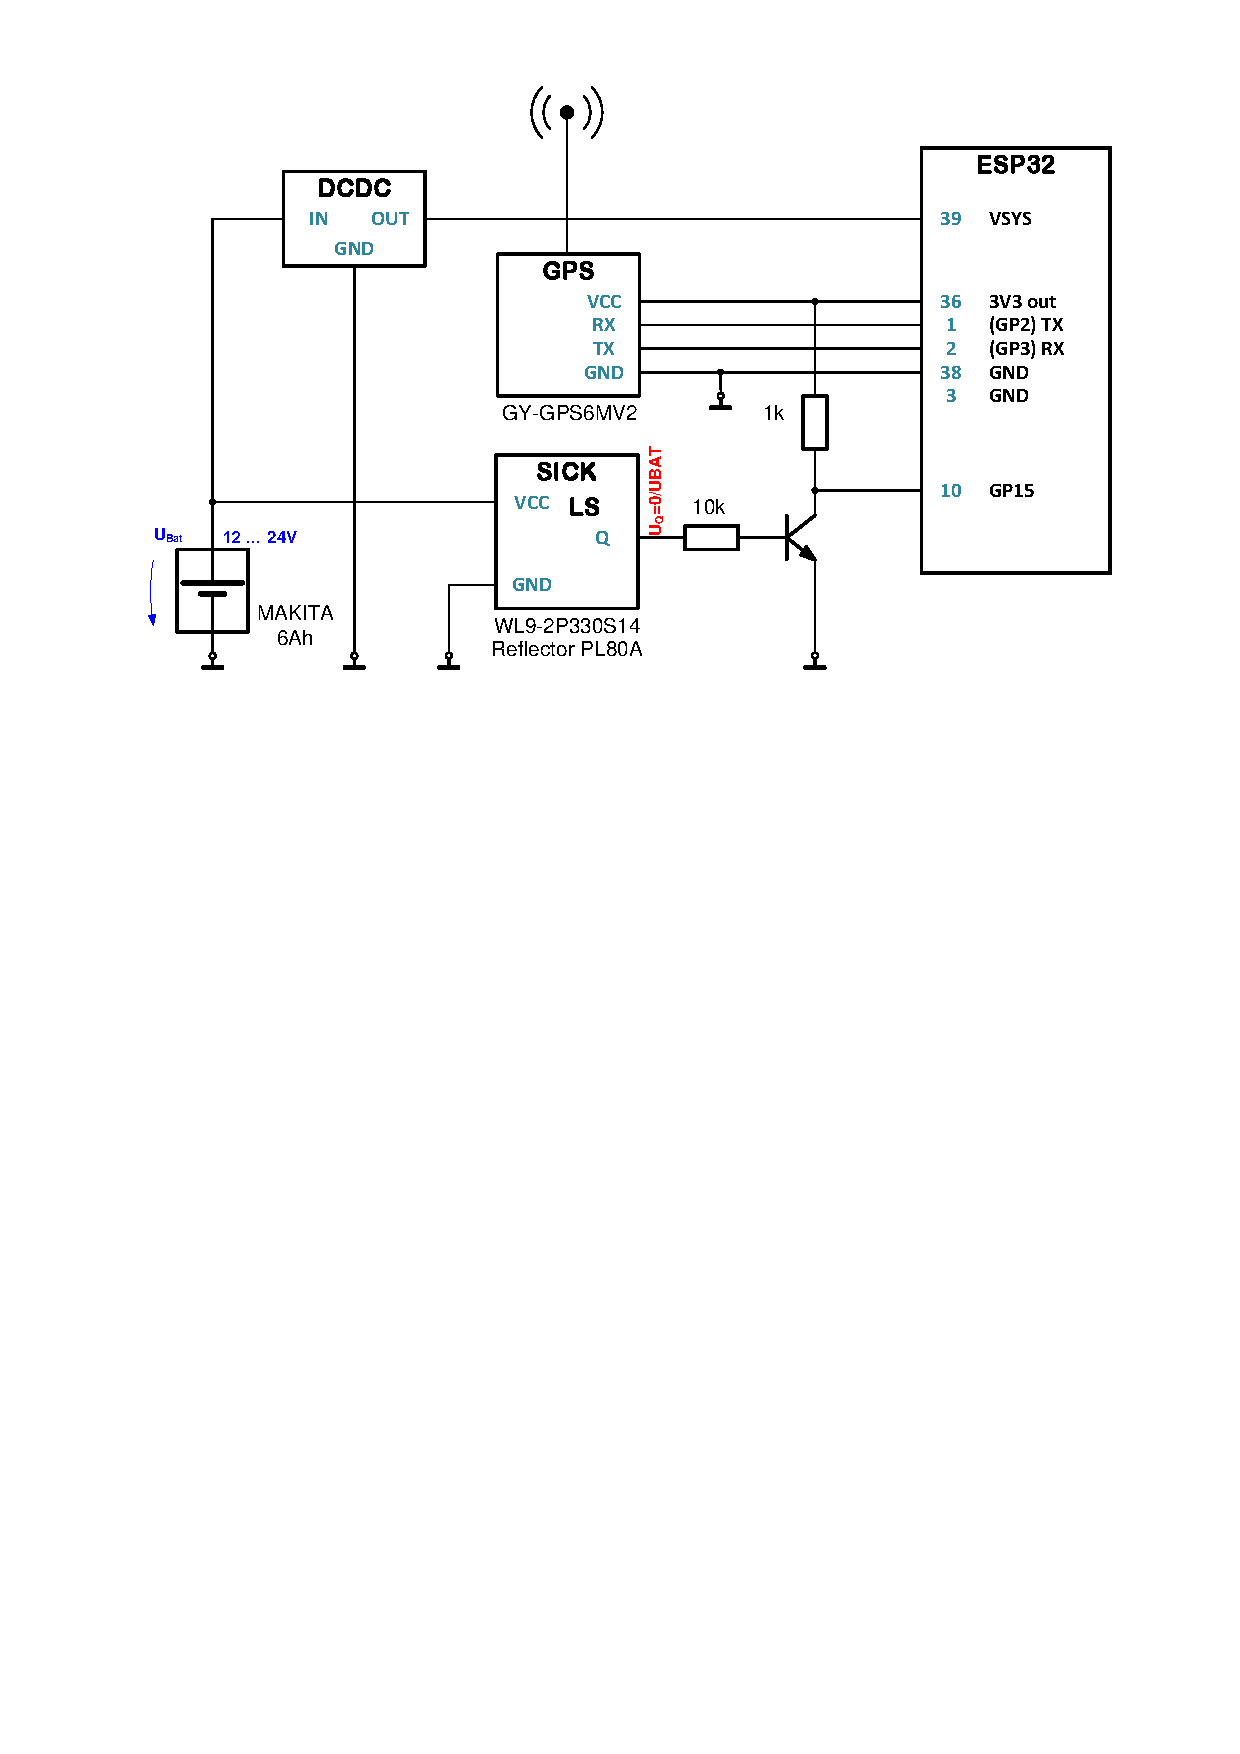
\includegraphics[width=\textwidth]{./01_Inhalte/06_Lichtschranke-Schaltplan.pdf}	
	\centering
	\caption{Lichtschranke-Schaltplan}
	\label{fig:Lichtschranke-Schaltplan}
\end{figure}


\subsection{MQTT}
Alle Zeitstempel werden über das WLAN mittels \textbf{MQTT} übertragen. Bei jedem Verbindungsaufbau mit dem MQTT-Broker wird im Topic \textbf{''clients''} der Name der Station übertragen \textbf{(''ESP32-'' + Mac-Adresse)}. Alle erfassten Zeitstempel der Lichtschranken-Stationen werden im Topic \textbf{''esp32/timestamps''} veröffentlicht. 

\subsection{Zeit-Synchronisierung}
Bei jedem Neustart oder erstmaligen Starten erfolgt eine Synchronisierung der Echtzeituhr (\ac{RTC}) mit dem GPS-Modul. Dies gewährleistet, dass jede Station über genau dieselbe Zeit verfügt.

\subsection{Lichtschranke}
Löst die Lichtschranke aus wird der \textbf{GPIO15-Pin} auf High (3,3V) gezogen. Softwaretechnisch löst dies eine \textbf{Interrupt-Routine } aus, in welcher die Zeit aus der \ac{RTC} auf Mikrosekunden genau ausgelesen wird. Im Loop wird dann dieser Zeitstempel weiterverarbeitet und am Display angezeigt bzw. an den MQTT-Broker gesendet.


\subsection{Implementierungsschritte}
Um das Programm auf den Arduino zu laden empfehle ich \textbf{Platformio} in VS-Code zu verwenden. In Platformio muss man den Projektordner ''\textbf{03\_LichtschrankenStation}'' öffnen. Zudem müssen einige Änderungen im Programmcode des ESP32 vorgenommen werden, damit der Code funktioniert. Grundsätzlich muss der Server sich im gleichem lokalem Netzwerk befinden wie die Lichtschranken-Stationen, somit muss die \textbf{SSID} \& das \textbf{Passwort} angepasst werden. Zudem muss man noch die \textbf{IP-Adresse} des Servers eintragen und die Benutzerdaten anpassen, falls diese geändert wurden. Diese Anpassungen müssen in der Datei \textbf{main.cpp}, die sich im Verzeichnis \textbf{/03\_LichtschrankenStation/src/} befindet, vorgenommen werden, um eine korrekte Verbindung zum Server zu gewährleisten.

\begin{lstlisting}[language=myCpp]
	// WiFi credentials
	const char* wifi_ssid = "SSID";          
	const char* wifi_password = "PASSWORD";  
	
	// MQTT server configuration
	const char* mqtt_server = "SERVER-IP";  
	const char* mqtt_user = "mqttclient";    
	const char* mqtt_password = "Kennwort1";  
\end{lstlisting}

Nach Durchführung dieser Modifikationen kann der Code kompiliert und auf den ESP32 geladen werden. Bevor man den Code auf den ESP32 lädt, musst man sicherstellen, dass das Gerät im Boot-Modus ist. Folgende Schritte müssen hierfür durchgeführt werden:

\begin{itemize}
	\item Schließe den ESP32 an den Computer an.
	\item Drücke und halte die BOOT-Taste, und drücke dann die RESET-Taste.
	\item Lasse zuerst die RESET-Taste los und dann die BOOT-Taste.
\end{itemize}

Da wir manuell den Boot-Modus aktiviert haben, wird bei der Übertragung eine Fehlermeldung auftauchen, die jedoch ignoriert werden kann. Nach Übertragung des Codes muss der ESP32 manuell neugestartet werden, indem man die \textbf{RESET-Taste} drückt.
\newpage


\section{\acl{GUI}}
\label{sec:GUI}

\begin{figure}[H]
	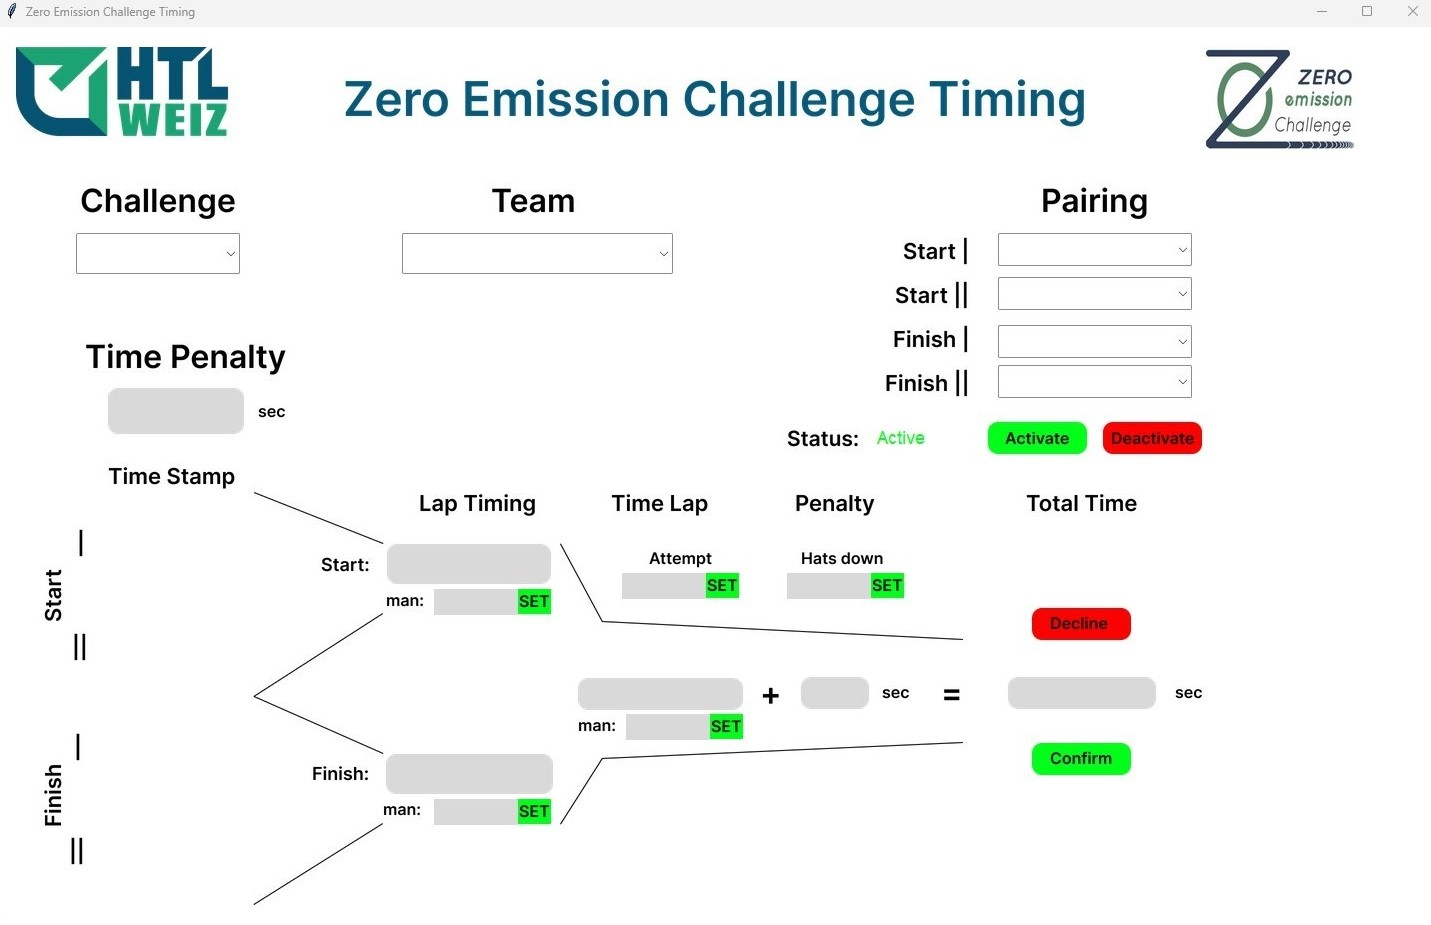
\includegraphics[width=\textwidth]{./01_Inhalte/13_GUI.jpg}
	\centering
	\caption{\ac{GUI}}
	\label{fig:GUI}
\end{figure}

Für die einfache Bedienung dieses Systems wurde eigens eine \ac{GUI} designend. Wie in Abbildung \ref{fig:GUI} zu sehen ist, kann man in der graphischen Benutzeroberfläche die aktuelle Challenge und Team, welche aus der \ac{DB} abgefragt werden, auswählen. Zudem können die verwendeten ESP32 für Start und Ziel ausgewählt werden. Auf der Bedienoberfläche werden von den ausgewählten ESP32 jeweils die letzten vier Zeitstempel angezeigt. Bei Auswahl von zwei Zeitstempeln für den Start bzw. des Ziel (Start | \& Start || oder Finish| \& Finish||), wird der Mittelwert der beiden Zeitstempel berechnet und für die Berechnung der Rundenzeit verwendet. Zudem kann der Start- oder Zielzeitstempel manuell im Format \textbf{hh:mm:ss.ssssss} eingeben und mit dem SET-Button gesetzt werden. Aus dem Start- sowie Finish-Zeitstempel wird die Rundenzeit berechnet, welche auch manuell im Format \textbf{s.ssssss} eingegeben und ebenfalls mit dem SET-Button gesetzt werden kann. Des Weiteren muss noch die Versuchsnummer (Attempt) als \textbf{Ganzzahl} und die umgefahrenen Hüttchen (Hats down) eingegeben werden. Die Zeitstrafe (Penalty) wird durch Multiplikation der \textbf{Hats down} mit dem \textbf{Time Penalty}, welcher auch aus der \ac{DB} entnommen wird, berechnet. Bei vollständiger Eingabe aller Felder bzw. Daten kann der \textbf{Confirm-Button} betätigt werden, wodurch der aktuelle Versuch des Teams in die Datenbank gespeichert wird. Bei Betätigung des \textbf{Decline-Buttons} werden bis auf das ausgewählte Team, Challenge und der ESP32 alle eingegeben Daten zurückgesetzt (das betrifft nicht die letzten vier Zeitstempel der ESP32). Abschließend sollte noch der Statusmodus erklärt werden. Dieser bietet die Möglichkeit Zeitstempel der ESP32 zu berücksichtigen (in der \ac{GUI} anzuzeigen) oder zu ignorieren.


\subsection{Implementierungsschritte}
Damit man die \ac{GUI} ausführen kann, muss man Python installieren. Wichtig ist hierbei das beim Setup-Vorgang \textbf{''Add python.exe to PATH''} angekreuzt wird, damit dem Betriebssystem mitgeteilt wird wo die Python-Interpreter-Datei (python.exe) zu finden ist. Danach muss man noch die benötigten Bibliotheken installieren. Hierfür muss man ein neues Terminal in VS-Code öffnen und folgenden Befehl ausführen damit die benötigten Pakete installiert werden:

\begin{Textfeld1}
	pip install -r ./02\_GUI/requirements.txt
\end{Textfeld1}

Wobei selbstverständlich hier der richtige, relative Pfad eingesetzt werden muss.
Um die Verbindung zwischen der \ac{GUI} und dem MQTT-Broker sowie dem \ac{DBMS} herzustellen, sind einige Anpassungen im \ac{GUI}-Code erforderlich. Es sind zwei wesentliche Änderungen erforderlich: Zum einen muss die \textbf{IP-Adresse} des Servers angepasst werden, und zum anderen müssen die \textbf{Benutzerdaten} in der Datei \textbf{gui.py}, die sich im Ordner \textbf{02\_GUI} befindet,  modifiziert werden. 

\begin{lstlisting}[language=Python]
	# Server configuration
	SERVER_IP = "IP-Address"       
	
	# MQTT configuration
	MQTT_USER = "mqttclient"       
	MQTT_PASSWORD = "Kennwort1"    
	
	# Database configuration
	DB_USER = "mariadbclient"      
	DB_PASSWORD = "Kennwort1"      
\end{lstlisting}

Wichtig ist zudem, dass der Ordern ''\textbf{assets}'' und die Datei ''\textbf{models.py}'' sich auf der gleichen Ordnern-Ebene wie das \ac{GUI}-Programm ''\textbf{gui.py}'' befindet.




\newpage

% 									Closing - Vorlage für Elektrotechnik
%                 					        2023 HTL Weiz
%----------------------------------------------------------------------------------------------------


%****************************************************************************************************
%========================================== A N H A N G =============================================
%****************************************************************************************************
%\newpage
%\addsec{Anhang}

%
\includepdf[pages=-]{./02_Documents/01_Sick-WL9-2P330S14.pdf}
%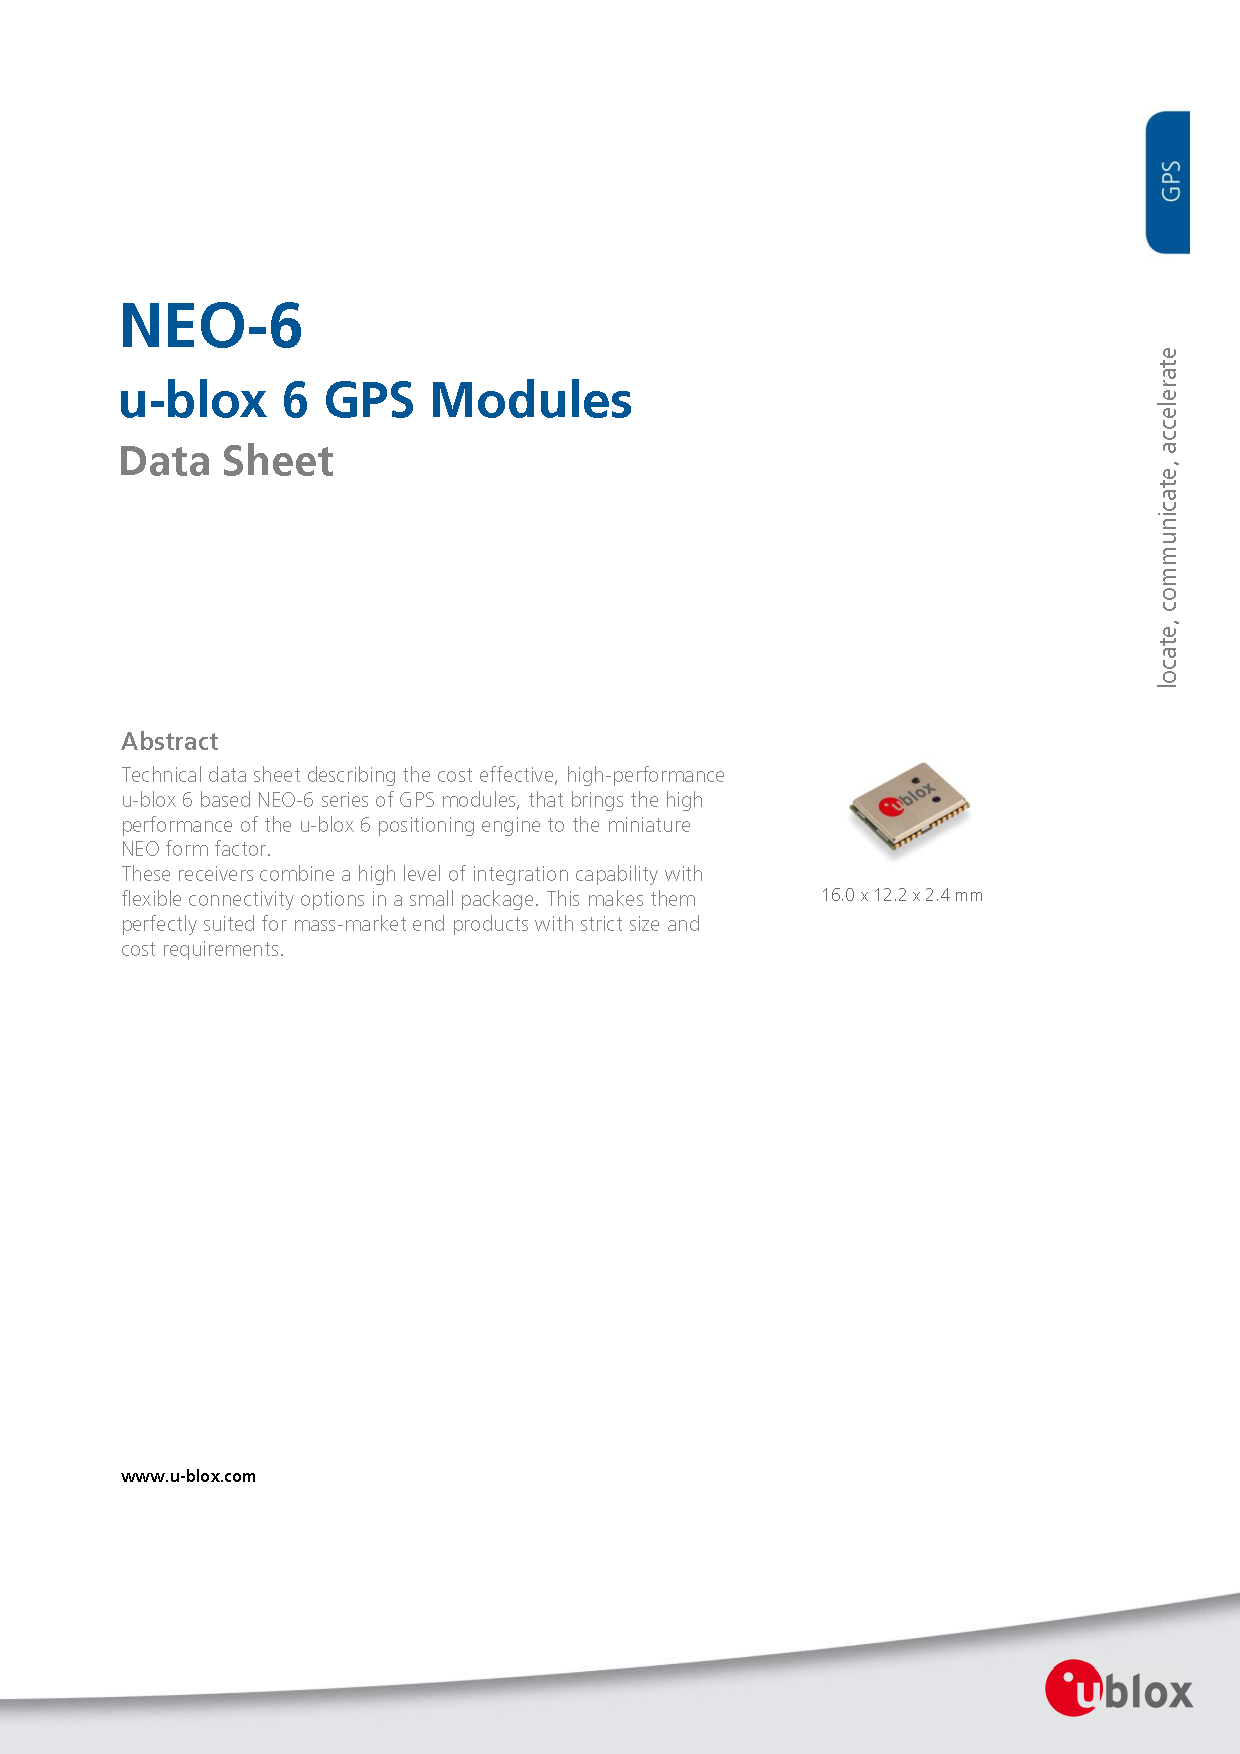
\includepdf[pages=-]{./02_Documents/02_UBlox-Neo-6MV2.pdf}
%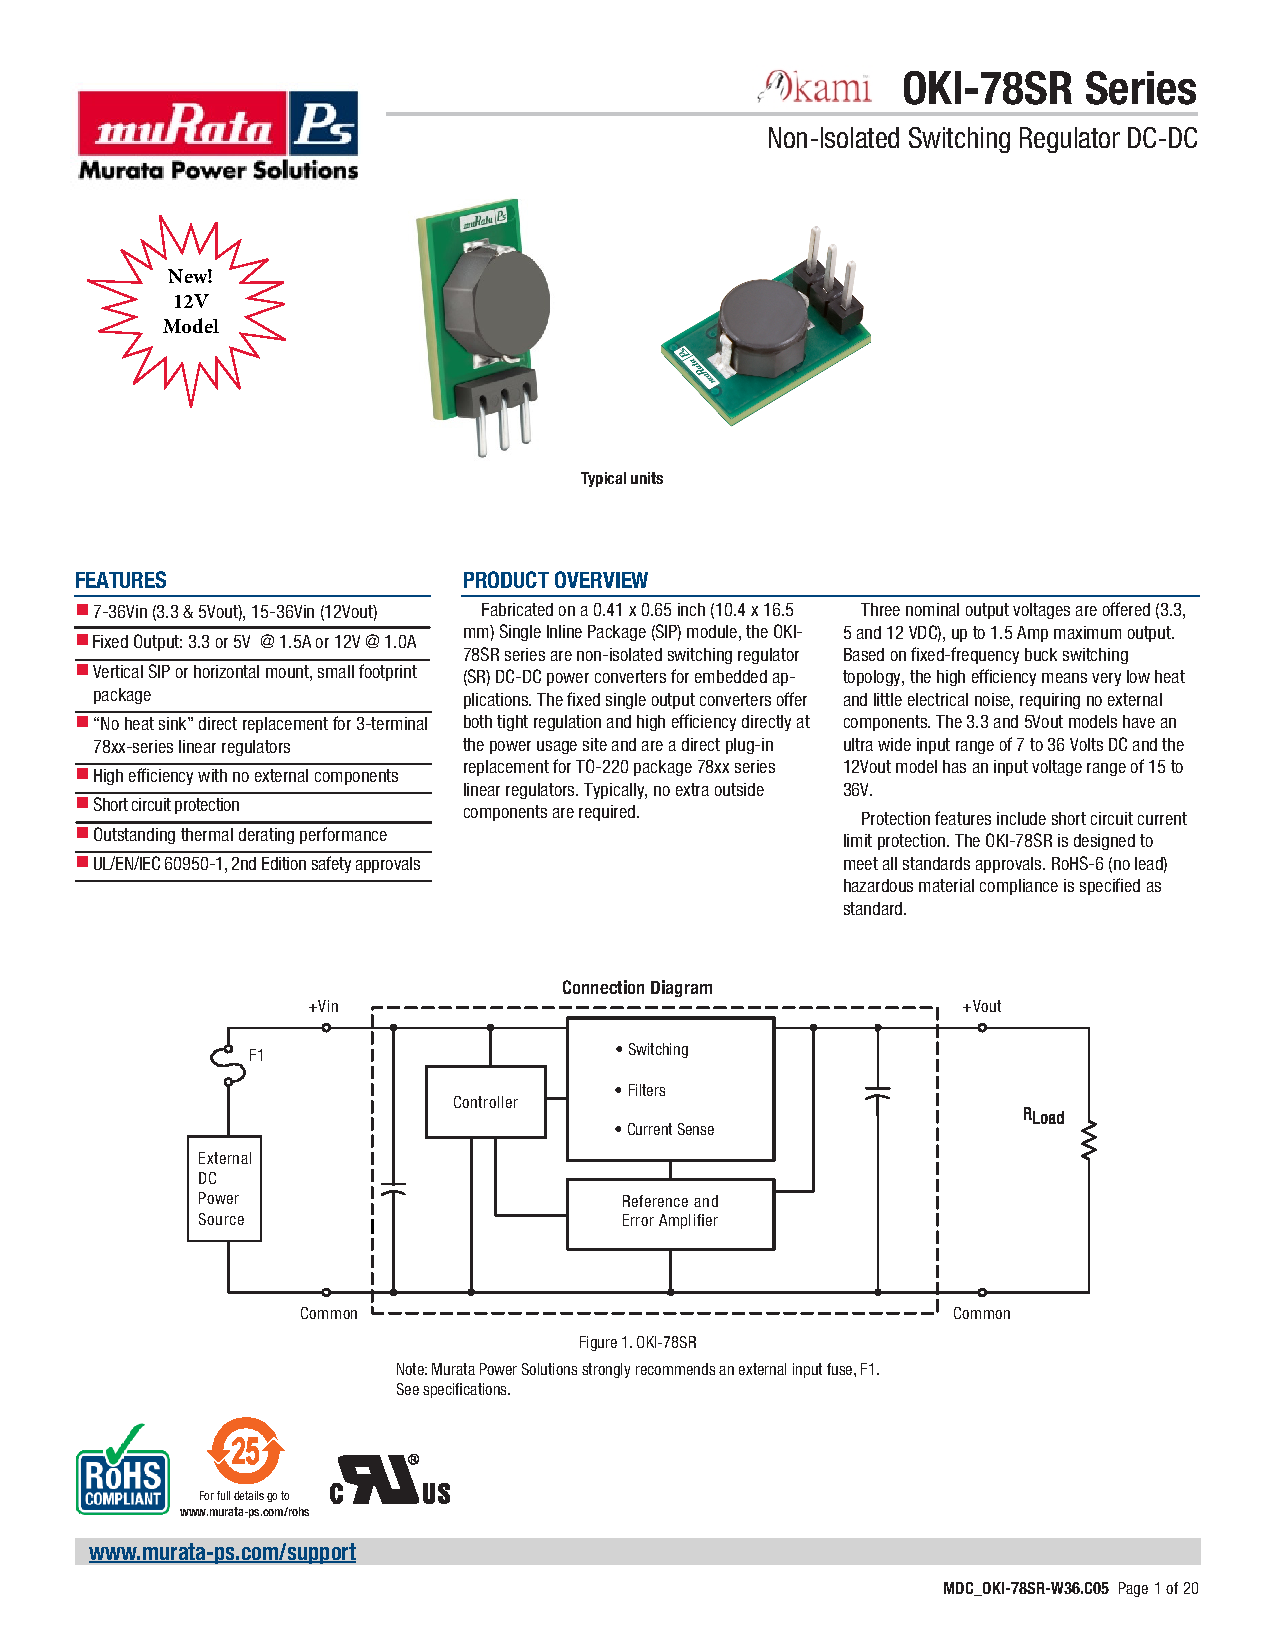
\includepdf[pages=-]{./02_Documents/03_Switching_Regulator.pdf}

%****************************************************************************************************
%============================ A B B I L D U N G S V E R Z E I C H N I S==============================
%****************************************************************************************************
\newpage
\listoffigures

%****************************************************************************************************
%============================= A B K Ü R Z U N G S V E R Z E I C H N I S ============================
%****************************************************************************************************
\newpage
\addsec{Abkürzungsverzeichnis}

\begin{acronym}[DBMS]	% Eckige Klammer: längste Abkürzung eintragen (Spalten werden angeglichen)
	\acro{DB}{Datenbank}
	\acro{GUI}{Graphical User Interface}
	\acro{DBMS}{Datenbank-Management-System}
	\acro{RasPi}{Raspberry Pi}
	\acro{DHCP}{Dynamic Host Configuration Protocol}
	\acro{µC}{Mikrocontroller}
	\acro{RTC}{Real Time Clock}
\end{acronym}


\newpage

%============================== L I T E R A T U R V E R Z E I C H N I S =============================

\printbibliography

\newpage


	
\end{document}

